\documentclass[11pt,a4paper,twoside,openright]{report}

%frontespizio
\providecommand{\coursename}{Progetto di Ingegneria Informatica}
\providecommand{\annoacc}{2013-2014}
\providecommand{\principaladviser}{Prof. Andrea Bonarini}
\providecommand{\firstauthor}{Davide Tateo}
\providecommand{\firstauthorid}{799311}
\title{Cognitive SLAM: Knowledge-Based Simultaneous Localization and Mapping}
\author{\firstauthor}

\usepackage{settings/frontesp}

\usepackage[italian]{hyperref}
\hypersetup{
    colorlinks,
    citecolor=black,
    filecolor=black,
    linkcolor=black,
    urlcolor=black
}
\newcommand{\autorefA}[1]{\hyperref[#1]{Algoritmo \ref{#1}}}

\usepackage{tabularx}
\usepackage{subfigure}
\usepackage{afterpage}
\usepackage{amsmath,amssymb}
\usepackage{amsthm}
\usepackage{settings/columnVectors}
\usepackage{rotating}  
\usepackage{fancyhdr}
\usepackage{algorithm}
\usepackage{algpseudocode}
\usepackage[epsilon]{backnaur}
\usepackage{tocbibind}
\usepackage[scriptsize]{caption} 
\usepackage{enumitem}
\usepackage{listings}
\usepackage{settings/languages}

\setlength{\oddsidemargin} {2. cm}
\setlength{\evensidemargin} {2. cm}
\addtolength{\oddsidemargin} {-0.4 cm}
\addtolength{\evensidemargin} {-0.4 cm}
\linespread{1.1}

\usepackage[italian]{babel}
\usepackage{lmodern}
\usepackage[utf8]{inputenc}
\renewcommand{\captionfont}{\normalfont \sffamily \itshape \small}

\setlength{\headheight}{15pt}
\pagestyle{empty}

\begin{document}
\pagenumbering{alph}
\titlep
\thispagestyle{empty} \normalfont \cleardoublepage
\vspace{17cm}

%\large
\begin{flushright}
\itshape{A mio papà\dots}
\end{flushright}

\thispagestyle{empty}  \cleardoublepage
\pagenumbering{roman}
\newpage
\chapter*{Sommario}

\addcontentsline{toc}{chapter}{Sommario}

Lo SLAM è uno dei principali problemi nello sviluppo di robot autonomi. Gli approcci correnti sono afflitti da un pesante costo computazionale e si comportano male in ambienti dinamici e disordinati; le performance di questi sistemi diventano ancora peggiori se si utilizzano sensori a basso costo, necessari per le applicazioni commerciali.
Questa tesi affronta il problema da un punto di vista nuovo e originale, usando feature ad alto livello come punti chiave e sfruttando la conoscenza di un esperto e un linguaggio fuzzy per riconoscerli, per tenere traccia di punti chiave forti e stabili e permettere mappe più intelligenti e una localizzazione robusta in ambienti complessi. L'idea fondamentale è quella di mantenere il tasso di errore della localizzazione limitato e ridurre il costo necessario a far navigare con successo un robot autonomo in un ambiente interno, usando solo i dati provenienti da una webcam e una unità di misura inerziale a basso costo.
Il principale problema è il riconoscimento di feature ad alto livello, come porte e scaffali, affrontato tramite un classificatore fuzzy ad albero, definito da un esperto, in modo da evitare fasi di allenamento e migliorare la generalità del riconoscimento.

\chapter*{Abstract}

\addcontentsline{toc}{chapter}{Abstract}

SLAM is one of the key issues in autonomous robots development. Current approaches are affected by heavy computational load and misbehave in cluttered and dynamic environment; their performance get even worse with low cost sensors, needed for market applications.
This thesis faces the problem in a new and original way, working with high level features as key points and using expert knowledge and a fuzzy language to detect them, in order to track strong and stable key points and allow smarter maps and robust localization in complex environments. The key idea is to keep the error rate of the localization process limited, and to reduce the cost of an autonomous robot to successfully navigate into an indoor environment using only the data from a webcam and a low cost Inertial measurement unit.
The main issue is the high level feature recognition, like doors and shelves, done by an expert-defined fuzzy tree classifier, in order to avoid training and improve generalization of recognition.
\thispagestyle{empty} \vspace*{.75truecm} \cleardoublepage
\tableofcontents
\listoffigures
\clearpage
\chapter*{Ringraziamenti}

\addcontentsline{toc}{chapter}{Ringraziamenti}

Dopo cinque lunghi anni, sono finalmente giunto al momento di scrivere i ringraziamenti. Questo significa che sono sopravvissuto al ``Vietnam'' che è il Politecnico! Un'esperienza entusiasmante e tremendamente difficile.

Non voglio utilizzare questa pagina per fare i soliti ringraziamenti scontati: il professore mi ha aiutato, la famiglia mi ha sostenuto... Beh, penso che queste cose, seppure vere, non siano i motivi fondamentali per cui valga la pena di spendere delle parole.

Piuttosto, voglio ringraziare il Professor Bonarini per avermi dato una sfida difficile da affrontare, una sfida che mettesse alla prova le mie capacità fino al limite e che mi ha permesso di imparare così tante cose che, se me lo avessero detto prima, non ci avrei creduto. Lo ringrazio perchè devo a lui, e ai suoi collaboratori (come il buon Martino!), tutte le cose che ho imparato e che fanno la differenza tra uno studente qualunque e un vero ingegnere.

Voglio ringraziare anche Davide Cucci, per il suo fondamentale aiuto nella parte di localizzazione, quando ormai credevo di doverla escludere dalla tesi (E comunque il telefono non ha suonato!).

Voglio ringraziare anche Andrea Romanoni per essere riuscito a rispondere alle mie domande anche sotto l'ombrellone!

Voglio ringraziare i ``Nerd della prima fila'' per essere riusciti a:
\begin{itemize}[noitemsep, nolistsep]
 \item Farsi sgridare dal proprio relatore.
 \item Farsi bersagliare da gessi.
 \item Farsi sgridare da persone a caso per il casino in aula studio.
 \item Fare battute sconvenienti.
 \item Riprodurre musica e filmati sconvenienti (sempre nelle aule studio, ovvio!).
 \item Aprire siti sconvenienti da usare come esempi di applicazioni.
 \item Farsi prendere in giro perfino dai prof per la ``nerditudine''.
\end{itemize}

Voglio sottolineare che io non c'entro ASSOLUTAMENTE niente con tutte queste malefatte! Ok\dots forse 2\dots 3\dots volte\dots

Voglio infine ringraziare la mia famiglia per avermi sempre amato. Forse avrei potuto arrivare qui dove sono ora e essere quello che sono ora senza il supporto economico, gli sforzi per permetterci di seguire le lezioni e tutto il necessario ad affrontare una università impegnativa come il Politecnico. Ma sicuramente non sarei arrivato da nessuna parte senza il loro affetto. Perchè la cosa che più importa in una famiglia è sapere che la tua famiglia ci sarà sempre e comunque per te, qualsiasi cosa accada, proprio perchè si è una famiglia. Vi voglio bene.

Grazie.

\thispagestyle{empty} \vspace*{.75truecm} \normalfont \cleardoublepage
\pagestyle{plain}\renewcommand{\chaptermark}[1]{\markboth{\chaptername\ \thechapter.\ #1}{}} 
\renewcommand{\sectionmark}[1]{\markright{\thesection.\ #1}}         
\fancyhead[LE,RO]{\bfseries\thepage}    
                                        
\fancyhead[RE]{\bfseries\leftmark}    
\fancyhead[LO]{\bfseries\rightmark}     
\renewcommand{\headrulewidth}{0.3pt} 
\pagenumbering{arabic}
\thispagestyle{plain}

\chapter{Introduzione}
\label{cap:Introduzione}
\thispagestyle{empty}

\begin{quotation}
{\footnotesize
\noindent{\emph{Doc: Sai sono stati gli scritti di Giulio Verne ad influenzare profondamente la mia esistenza. Avevo 11 anni quando ho letto per la prima volta ``Ventimila leghe sotto i mari''. E' stato allora che ho capito che dovevo dedicare la mia vita alla scienza!
}
}
\begin{flushright}
Ritorno al Futuro, parte III
\end{flushright}
}
\end{quotation}
\vspace{0.5cm}

Uno dei problemi chiave della robotica è la localizzazione di un robot in un ambiente sconosciuto. Questo problema è noto come ``SLAM'', Simultaneus localization and Mapping, ed è attualmente una delle aree più importanti della ricerca riguardante i robot autonomi. 
In particolare, questo problema risulta ancora più difficile se applicato a robot dotati di sensori a basso costo, quali webcam e unità di misura inerziale economiche, restrizione fondamentale per la diffusione di applicazioni di robotica autonoma nel mondo reale. \\
Attualmente questo problema è affrontato attraverso tecniche probabilistiche, che sono ottime per analizzare ambienti statici e per ottenere una localizzazione precisa. Le mappe create sono utilizzabili principalmente per la navigazione.
I sensori più usati sono gli scanner laser, che tuttavia sono molto costosi, i sensori RGB-D, sensori economici che nascono per applicazioni videoludiche commerciali e hanno alcune limitazioni se applicati alla robotica, le telecamere stereo. \\
Lo scopo della tesi è di sviluppare un framework per risolvere il problema della localizzazione di robot autonomi dotati di sensori a basso costo, quali ad esempio i quadricotteri. L'idea è di sviluppare una metodologia che non solo permetta al robot di localizzarsi nella mappa in maniera efficiente, ma anche di interagire con l'ambiente in maniera avanzata, di compiere ragionamenti, di adattarsi a eventuali cambiamenti ed agli eventi che possono occorrere, quali la presenza di persone o altri agenti. \\
Basandosi principalmente sulle informazioni provenienti da una videocamera monoculare, è stato sviluppato un sistema che è in grado di processare informazioni provenienti da un esperto, espresse in un linguaggio formale, di estrarre feature di basso livello e aggregarle, grazie alla base di conoscenza, per riconoscere e tracciare feature di alto livello, quali porte e armadi, e di basare conseguentemente su di essi il processo di localizzazione.
Per permettere all'esperto di trasmettere la sua conoscenza all'agente, è stato sviluppato un linguaggio formale, basato sulla logica fuzzy, che permetta sia di esprimere regole fuzzy linguistiche, sia di definire un classificatore fuzzy ad albero in grado di definire una gerarchia di modelli e le relazioni tra di essi. \\
Infine si utilizzano tecniche avanzate di fusione multisensoriale e localizzazione per estrarre la posizione del robot e degli oggetti nell'ambiente esplorato.

\noindent
La tesi è strutturata nel modo seguente: \\
Nel \autoref{cap:statoArte} si illustra lo stato dell'arte. \\ 
Nel \autoref{cap:architettura} si descrive l'architettura generale del sistema. \\
Nel \autoref{cap:reasoning} si parla del reasoner e del linguaggio formale utilizzato. \\
Nel \autoref{cap:riconoscimento} si descrive il riconoscimento degli oggetti \\
Nel \autoref{cap:tracking} si mostra come gli oggetti riconosciuti sono tracciati. \\
Nel \autoref{cap:mapping} si illustra la creazione della mappa e la localizzazione. \\
Nel \autoref{cap:risultati} si analizzano i risultati sperimentali del sistema proposto. \\
Nel \autoref{cap:sviluppi} si riassumono gli scopi, le valutazioni di questi e le prospettive future. 


\chapter{Stato dell'arte}
\label{cap:statoArte}
\thispagestyle{empty}

\begin{quotation}
{\footnotesize
\noindent{\emph{Doc: Ecco perché non ha funzionato: c'è scritto ``Made in Japan''. \\
Marty: E che vuol dire Doc? Tutta la roba migliore è fatta in Giappone. \\
Doc: Incredibile!
} }
\begin{flushright}
Ritorno al Futuro, parte III
\end{flushright}
}
\end{quotation}
\vspace{0.5cm}

\section{SLAM}

Il problema della localizzazione di un robot e costruzione della mappa in contemporanea in un ambiente sconosciuto è stato affrontato fin dagli anni '90 a partire da~\cite{174711}, articolo nel quale per la prima volta si delineava un framework per localizzare un robot costruendo contemporaneamente la mappa dell'ambiente.

Tramite l'utilizzo di sonar, venivano estratte feature geometriche con cui veniva costruita la mappa, nella quale il robot si localizzava. 
Il problema principale della localizzazione è il ``problema della correlazione'': se la posizione della feature rispetto alla quale ci si localizza è affetta da incertezza, la conseguente stima della posizione effettuata rispetto a tale feature sarà affetta da un errore che dipende dall'errore della posizione della feature stessa. 
Questo problema diventa tanto più grave se si pensa che la posizione del robot in ogni istante non è nota a priori, ma deve essere stimata sulla base delle osservazioni precedenti. 

\`E necessario risolvere questo problema per evitare che l'errore della generazione della mappa e l'errore della stima della posizione divergano nel tempo. 
Per risolverlo, gli autori hanno spesso utilizzato un filtro di Kalman esteso.

Il filtro di Kalman è uno stimatore Bayesiano ricorsivo, che, supposto noto il modello lineare che regola la generazione dei dati e la loro osservazione, supposto che l'errore di misura e di modello siano gaussiani, restituisce la densità di probabilità del sistema osservato. 
Il filtro di Kalman, se utilizzato secondo le ipotesi, è uno stimatore ottimo dello stato del sistema osservato, secondo i minimi quadrati.
Tuttavia, nell'ambito della robotica, e in particolare nel problema della localizzazione, il modello di generazione e osservazione dei dati non può essere considerato lineare.
E' quindi necessario utilizzare un'estensione del filtro di Kalman al caso non lineare: il filtro di Kalman esteso (EKF) è una delle possibili soluzioni al problema. 
L'idea alla base del filtro di Kalman esteso è quella di lavorare sul modello linearizzato, stimato ricorsivamente dal modello non lineare sulla base della stima corrente.

Per avere una buona stima della posizione è necessario utilizzare un gran numero di feature, numero che cresce molto rapidamente con l'aumentare della dimensione dell'ambiente.
La complessità computazionale dell'approccio tradizionale basato sul filtro di Kalman esteso è $\mathcal{O}(N^3)$, con $N$ numero di feature, e quindi il tempo di calcolo diventa ben presto inaccettabile per prestazioni in tempo reale.
Per risolvere questo problema è stato introdotto in~\cite{Montemerlo02a} un nuovo algoritmo detto FastSLAM, che consiste nell'utilizzo del Particle Filter, e del filtro di Kalman esteso in combinazione. L'algoritmo associa ad ogni feature considerata, un filtro di Kalman esteso; la densità di probabilità congiunta, invece, viene calcolata sfruttando il Particle filter. 
Il Particle Filter è un altro stimatore Bayesiano ricorsivo, che, invece di un modello e dell'assunzione di rumore gaussiano, sfrutta metodi di tipo Monte Carlo per stimare la densità di probabilità del sistema che genera i dati.
Il risultato è un algoritmo che ha complessità computazionale $\mathcal{O}(N\log M)$, con $M$ numero di feature e $N$ il numero di particelle usate dal Particle Filter. 
Questo approccio rende il problema trattabile nella maggior parte dei casi, pur essendo pesante computazionalmente, dato che è necessario un elevato numero di particelle per avere una buona localizzazione.

Vista la particolarità del problema quando il sensore utilizzato è una videocamera monoculare, sono stati sviluppati algoritmi ad hoc.
Uno degli algoritmi più usati è PTAM~\cite{klein07parallel},~\cite{klein08improving}.
L'idea alla base di questo algoritmo è dividere in due thread separati il tracking e la creazione della mappa: un thread si occupa del tracking robusto di feature a basso livello, mentre l'altro thread si occupa della creazione della mappa. 
Per rendere efficiente il processo di mapping, solo i keyframe, ossia i frame che contengono maggiore informazione rispetto a quella già presente, vengono considerati.
Per rendere il processo di mapping robusto, vengono utilizzate tecniche batch per costruire la mappa, come ad esempio il bundle adjustment. Il bundle adjustment consiste in un processo iterativo di raffinamento della stima dei punti 3D ricostruiti e della posa della videocamera.
PTAM, tuttavia, nasce per applicazioni di realtà aumentata, e quindi necessita di una inizializzazione, per risolvere i problemi dell'acquisizione del primo keyframe e per gestire la scala della mappa.

Un approccio alternativo consiste nell'usare tutti i dati dell'immagine per eseguire la localizzazione, questo approccio è alla base, ad esempio, di DTAM, Dense Tracking and Mapping~\cite{conf/iccv/NewcombeLD11}. Questo algoritmo crea un modello denso dell'ambiente e usa l'allineamento della videocamera

Si sono dimostrati efficaci anche i metodi semi-diretti, come SVO~\cite{Forster2014ICRA}, Semi Direct Visual Odometry, un algoritmo che riesce a ottenere altissime prestazioni limitando l'estrazione delle feature ad alto livello ai soli keyframe, operando direttamente sulle intensità dei pixel nei frame successivi, eliminando le fasi computazionalmente più onerose, che sono l'estrazione e l'abbinamento delle feature. SVO si basa sulle idee di PTAM, ma ne migliora sia le prestazioni, riuscendo a essere computazionalmente più leggero, sia la precisione della mappa e della localizzazione riducendo di molto gli outlier.

Recentemente, stanno avendo molto successo i sistemi basati su sensori RGB-D~\cite{izadi2011kinectfusion},~\cite{henry2012rgb}. Questi sensori vengono utilizzati come scanner laser a basso costo per creare una mappa dell'ambiente. Tuttavia, sono soggetti a molte limitazioni, non essendo stati progettati per questo scopo, e soffrono tra l'altro di un raggio d'azione limitato. Nonostante queste limitazioni i sistemi riescono comunque a ottenere buone prestazioni in ambienti indoor~\cite{sturm2012benchmark}.

\section{Rappresentazione del Mondo}

Sono noti diversi modi per rappresentare un ambiente tridimensionale.
Il più semplice possibile è quello di usare delle nuvole di punti, direttamente estratte dai sensori. Un'altra rappresentazione comune è quella di filtrare le nuvole di punti ottenute tramite una griglia di voxel, come, ad esempio, in~\cite{30724}.
Metodi più avanzati permettono una rappresentazione geometrica dell'ambiente con un minor uso di memoria, come, ad esempio, le mappe di quota, in cui una mappa a due dimensioni è estesa con il calcolo del valore medio di altezza di ciascun punto 2D~\cite{herbert1989terrain}, le mappe di quota estese~\cite{pfaff2007efficient}, che tengono conto di possibili aperture attraversabili dai robot, oppure le mappe di quota multi livello~\cite{4058725}, che riescono a descrivere complesse geometrie multi livello.

Tra le mappe più promettenti esistono le mappe basate sugli octree, che permettono un'efficiente rappresentazione in memoria sia dello spazio occupato sia dello spazio libero, pur potendo descrivere geometrie complesse. Inoltre, questo tipo di rappresentazione permette di scalare facilmente la risoluzione della mappa, permettendo di utilizzare la stessa mappa per compiti che richiedono una precisione differente.
Un'efficiente implementazione di questo tipo di mappa può essere trovata in \cite{hornung13auro}.

Recentemente, si sta sviluppando l'idea di rappresentare il mondo ad alto livello, incorporando informazioni semantiche e geometriche che possano essere utilizzate non solo dagli algoritmi di navigazione, ma anche per svolgere compiti ad alto livello e ragionamenti. Una possibile soluzione al problema è l'approccio basato su Scene Graph~\cite{6630614}. Sono stati sviluppati anche linguaggi specifici di dominio (DSL) per poter interagire ad alto livello, ad esempio generando istanze di oggetti a partire da un modello generico, come ad esempio in \cite{blumenthal2014towards}.

\section{Riconoscimento di Oggetti}

La quasi totalità degli algoritmi di riconoscimento di oggetti nell'immagine è basata su tecniche di machine learning.
Una delle classi di algoritmi più usati sono quelli basati sulle Haar-like feature~\cite{710772}.
Queste feature sono calcolate in aree rettangolari, all'interno delle quali vengono sommati i valori dell'intensità dei pixel. Le somme sono in seguito usate per calcolare differenze tra aree di interesse, per poter riconoscere feature geometriche quali angoli, linee o bordi.
Un efficiente algoritmo per il riconoscimento di oggetti è descritto in~\cite{Viola01rapidobject} ed è stato ampliato in~\cite{Lienhart02anextended}, e consiste nell'utilizzare in cascata una serie di classificatori via via più restrittivi; ognuno dei classificatori di ogni stadio è costruito attraverso una tecnica di boosting, ossia sono formati da un insieme di classificatori deboli che creano un classificatore complessivo più restrittivo. I classificatori di base sono solitamente alberi di decisione. Il classificatore complessivo dà una risposta binaria; per riconoscere effettivamente l'oggetto deve essere applicato tramite una finestra mobile su tutta l'immagine. \\
Un algoritmo simile è descritto in~\cite{journals/ijista/AbramsonSG07}, dove, però, invece che feature Haar-like, vengono utilizzati direttamente un insieme di pixel selezionati nell'immagine.

Un'altra importante classe di algoritmi è basata sulle feature HOG (Histogram of Oriented Gradients)~\cite{1467360}.

Queste feature sono ricavate contando le occorrenze dell'orientamento dei gradienti in sotto-blocchi dell'immagine.
Su queste feature si basa l'algoritmo descritto in~\cite{lsvm-pami}. Questo algoritmo è in grado di definire un oggetto a partire dalle sue parti, e quindi è robusto anche a occlusioni parziali dell'oggetto. Tuttavia è computazionalmente molto più pesante dell'approccio basato su feature Haar-like.

Più recenti sono i metodi basati sul deep learning. Tra questi, i più promettenti nel riconoscimento di oggetti sono basati sulle reti neurali convoluzionali. La particolarità di queste reti è di essere basata su kernel di nodi collegati in maniera fissa, e ripetuti per coprire tutta l'immagine. La struttura rigida sfrutta la località dell'informazione nell'immagine, e permette un training più efficiente.
Un esempio di applicazione si può trovare in~\cite{NIPS2012_4824}.

Metodi recenti, sfruttano sensori RGB-D, come ad esempio Kinect, per riconoscere oggetti nella scena, come ad esempio in~\cite{lai2012detection}. La maggior parte delle tecniche usate sono un'estensione delle tecniche già descritte, spesso estendendo i descrittori delle feature grazie alle informazioni sulla profondità.

\section{Reasoning}

I sistemi di ragionamento sono stati alla base dell'Intelligenza Artificiale fin dalla nascita ed hanno trovato sbocco in diverse applicazioni tra cui i sistemi esperti, per lungo tempo una delle branche dell'intelligenza artificiale più attive~\cite{buchanan1984rule}~\cite{davis1977production}~\cite{joseph1994riley}.

Con la maturazione della tecnologia per lo sviluppo dei sistemi esperti, e l'avvento di Internet, l'attenzione della ricerca collegata ai sistemi di ragionamento formale si è spostata dai sistemi esperti al web semantico.
Il linguaggio più diffuso per i sistemi di inferenza è il linguaggio OWL 2~\cite{owl2-overview},~\cite{owl2-primer}, fortemente basato sulle logiche descrittive che permettono un buon compromesso tra espressività, e complessità computazionale e mantengono la logica utilizzata decidibile.

Fin dai primi sistemi esperti si è riconosciuta l'importanza del trattamento dell'incertezza in sistemi di ragionamento che avessero a che fare con il mondo reale~\cite{davis1977production}, ed in particolare si è avuta una larga diffusione in moltissimi settori della logica fuzzy~\cite{Zadeh1965338}, adottata anche nel nostro lavoro.

Un esempio di reasoning applicato al riconoscimento delle immagini può essere trovato in~\cite{DBLP:journals/ivc/MaillotT08}, in cui feature a basso livello vengono estratte da un meccanismo di machine learning, e utilizzate da un sistema di inferenza che sfrutta una ontologia per l'analisi ad alto livello dell'immagine. Un altro esempio di utilizzo di sistemi di inferenza nel riconoscimento di oggetti si può trovare in~\cite{DBLP:journals/corr/abs-1301-4991}, dove viene utilizzato il linguaggio OWL per specificare una base di conoscenza e riconoscere tramite la conoscenza di dominio gli oggetti nell'ambiente.


\chapter{Architettura del Sistema}
\label{cap:architettura}
\thispagestyle{empty}

\begin{quotation}
{\footnotesize
\noindent \emph{Doc: Questo rende possibile viaggiare nel tempo... il flusso canalizzatore.
Marty: Flusso canalizzatore?! \\
Doc: Mi ci sono voluti quasi 30 anni e tutto il mio patrimonio per realizzare la visione di quel giorno... mio Dio quanto tempo è passato! \\
\dots \\
Marty: Questa... questa è proprio forte Doc! E' grande! Ma funziona con la benzina normale? \\
Doc: Sfortunatamente no! Ha bisogno di un qualcosa di un po' più vivace: Plutonio.
}
\begin{flushright}
Ritorno al Futuro, parte I
\end{flushright}
}
\end{quotation}
\vspace{0.5cm}

\section{Introduzione}
In questo capitolo descriveremo l'architettura del sistema, sia dal punto di vista logico, descrivendo la struttura della soluzione presentata, sia dal punto di vista dei moduli software, descrivendo nello specifico come è implementato il sistema, come comunicano i moduli implementati e quali tecnologie sono state utilizzate.

Il sistema implementato è pensato per risolvere il problema della localizzazione ad alto livello, cercando di riconoscere oggetti nell'immagine, anziché feature estratte dall'immagine come keypoint, linee o altri tipi di descrittori a basso livello, che possono essere facilmente confusi. Utilizzare oggetti noti nell'immagine, permette di estrarre conoscenza ulteriore sulle caratteristiche spaziali dell'ambiente, dato che le dimensioni dell'oggetto possono essere note, almeno in maniera approssimata. Inoltre, il nostro approccio permette di creare mappe semantiche sulle quali è possibile fare inferenze di vario tipo, inferenze che possono essere sfruttate anche per migliorare la navigazione stessa.

\section{Architettura Logica}
Per risolvere il problema descritto, abbiamo ritenuto necessario sviluppare i seguenti moduli:

\begin{itemize}
 \item Un reasoner in grado di analizzare dati e classificare feature.
 \item Un algoritmo di individuazione dei possibili oggetti interessanti.
 \item Un algoritmo di tracking che segua gli oggetti interessanti.
 \item Un algoritmo di riconoscimento degli oggetti individuati come interessanti, cercando di raffinare la classificazione.
 \item Un algoritmo che utilizzi le feature ad alto livello estratte per localizzare il robot nella mappa.
\end{itemize}

La struttura logica del sistema implementato è rappresentata in \autoref{fig:logica-sistema}.

\begin{figure}[ht]
  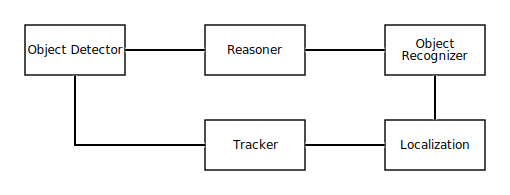
\includegraphics[width=\textwidth]{diagrammi/SchemaLogico}
  \caption{Schema logico del sistema}
  \label{fig:logica-sistema}
\end{figure}

\subsection{Individuazione degli oggetti}
L'individuazione degli oggetti è la base di partenza per l'estrazione dei punti di riferimento su cui si basa la localizzazione.
\`E in grado di analizzare un'immagine generica e di estrarre i possibili oggetti significativi.
Non è necessario che il riconoscimento di basso livello sia in grado di distinguere efficacemente le diverse classi di feature cercate, poiché l'analisi approfondita della feature verrà effettuata da altri sottosistemi; questa fase del riconoscimento è progettata per estrarre poca informazione, abbastanza per individuare le feature geometriche di base interessanti.
L'individuazione degli oggetti dipende fortemente dal sistema di reasoning.
Questo sottosistema è descritto nel \autoref{cap:riconoscimento}.

\subsection{Reasoner}
Il reasoner è il cuore del sistema ed è in grado di analizzare dati rumorosi e incerti e classificare istanze di possibili oggetti trovati dagli algoritmi di estrazione delle feature. Per poter svolgere questo compito in maniera efficace, e per poter affrontare in maniera rigorosa le incertezze, si è deciso di utilizzare un reasoner basato sulla logica fuzzy.
Per poter classificare oggetti il reasoner è in grado di utilizzare una knowledge base che contiene sia le classi che descrivono gli oggetti, sia le informazioni per interpretare in maniera simbolica i descrittori delle feature, che sono dati numerici. 
Poiché gli oggetti nel mondo reale sono definiti in base alle relazioni con gli altri oggetti, il reasoner è in grado di analizzare queste relazioni per permettere di compiere classificazioni avanzate.
Il reasoner è descritto nel \autoref{cap:reasoning}.

\subsection{Tracker}
Il tracker deve essere in grado di tracciare oggetti complessi, che possono uscire dall'immagine o essere parzialmente coperti. Per questo abbiamo implementato il tracker utilizzando un algoritmo di tracking a lungo termine. Grazie a questo tipo di algoritmi non è necessario avere un alto tasso di recupero per il sistema di individuazione degli oggetti, in quanto l'oggetto inseguito viene individuato automaticamente e con un buon tasso di confidenza nell'immagine. Grazie al tracker a lungo termine, possiamo associare con alta confidenza una determinata track a un punto di riferimento nell'algoritmo di localizzazione.
Poiché lo scopo del sistema è di utilizzare la massima informazione possibile in maniera intelligente, l'algoritmo di tracking è in grado di ricevere informazione dalla mappa e processarla per aumentare le sue prestazioni.
L'algoritmo di tracking è descritto nel \autoref{cap:tracking}.


\subsection{Riconoscimento degli oggetti}
Lo scopo di questo sottosistema è quello di implementare un algoritmo di riconoscimento di oggetti ad alto livello. Sfrutta l'informazione proveniente dal tracker per limitare l'analisi di immagine a una regione di interesse la più ristretta possibile, per aumentare le prestazioni sia computazionali sia di riconoscimento. L'informazione estratta da questo nodo può essere utilizzata per etichettare i punti di riferimento nella mappa o per aiutare la localizzazione, fornendo informazioni ulteriori all'algoritmo di localizzazione.
Il riconoscimento degli oggetti è descritto nel \autoref{cap:riconoscimento}.

\subsection{Localizzazione}
La localizzazione è effettuata utilizzando tutta l'informazione estraibile dai sensori e dal resto del sistema.
Il sottosistema che si occupa della localizzazione è in grado quindi di leggere i dati dai sensori del robot e utilizzare i dati estratti dal sistema di riconoscimento delle feature per creare una mappa e cercare di localizzarsi nella maniera più robusta possibile.
Il sistema di localizzazione è pensato per poter utilizzare sia l'informazione proveniente dal tracker, sia l'informazione proveniente dal riconoscimento degli oggetti.
Parleremo della localizzazione nel \autoref{cap:mapping}.

\section{Architettura Software}
Il sistema è stato progettato in maniera modulare per una serie di motivi: questo tipo di architettura permette di riutilizzare i moduli sviluppati, di estendere semplicemente il sistema con altri moduli, di sostituire eventualmente un intero modulo con un altro che compia le stesse funzioni, di comunicare in maniera semplice con altri sistemi. 

Per raggiungere questo scopo, si è deciso quindi di utilizzare il middleware ROS (Robot Operating System)~\cite{quigley2009ros}.
ROS è un middleware che, oltre ad offrire molti strumenti utili per lo sviluppo di complesse applicazioni robotiche, implementa due pattern architetturali importanti, entrambi usati nel nostro lavoro: il pattern publish-subscribe e il pattern client-server.
Questi due pattern sono implementati rispettivamente tramite messaggi e servizi: i messaggi definiscono un formato comune per la pubblicazione di dati in topic, i servizi invece specificano un'interfaccia per le chiamate a procedure remote, dichiarando gli input e gli output tra client e server.

Ogni processo che viene eseguito in ROS è chiamato nodo. Per eseguire qualsiasi sistema basato su ROS, devono essere presenti tre ulteriori nodi: il nodo Master, che si occupa di garantire la comunicazione tra gli altri nodi, tramite i due pattern supportati, il server dei parametri, che implementa un dizionario condiviso accessibile tramite la rete, in cui i nodi possono memorizzare e recuperare parametri usati dai loro algoritmi a runtime, il nodo \textit{rosout}, che si occupa di mantenere i log prodotti dalle applicazioni.

Il sistema sviluppato è pensato per interagire con qualsiasi tipo di robot che sia provvisto di una videocamera monoculare e una unità di misura inerziale (IMU), e eventualmente, un magnetometro, tramite le tre interfacce standard di ROS.
Esse consistono in quattro topic: ``imu'', per i dati provenienti dall'unità di misura inerziale, ``image\_raw'', per l'immagine proveniente dalla videocamera, ``camera\_info'', che contiene i parametri intrinseci della videocamera, tra cui la matrice di calibrazione della videocamera utilizzata, necessaria per il funzionamento del sistema, ``mag'' per i dati provenienti dal magnetometro.
I dati estratti dall'unità di misura inerziale devono poter essere riferiti al sistema di coordinate della videocamera, dato che l'algoritmo di visione implementato utilizza i dati provenienti dalla IMU per stimare approssimativamente la posa della telecamera.
Per rendere l'algoritmo portabile, si utilizza a libreria tf di ROS. La libreria tf gestisce le trasformazioni da un sistema di coordinate all'altro, pubblicando un albero di trasformazioni nel topic ``tf''.
Negli header dei messaggi standard di ROS è definito il campo ``frame\_id'', che descrive il nome del sistema di coordinate rispetto al quale è riferito il contenuto del messaggio. Grazie a questo, è possibile riferire i dati della IMU rispetto alle coordinate dell'immagine, purché sia nota la trasformazione tra i due frame.

\subsection{Diagramma del sistema}

\begin{figure}[ht]
  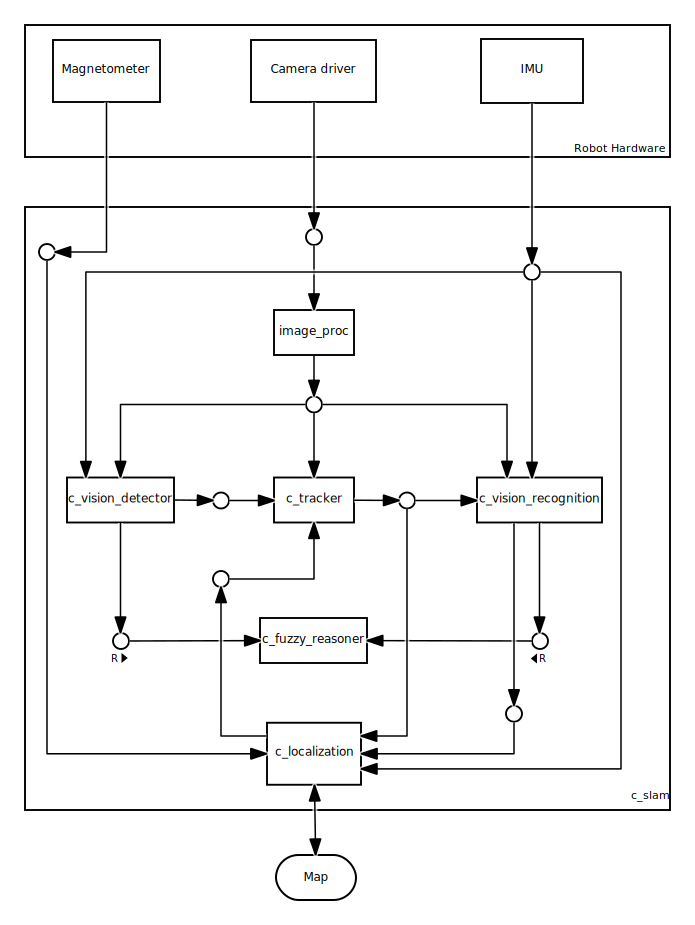
\includegraphics[width=\textwidth]{diagrammi/Sistema}
  \caption{Architettura del sistema implementato}
  \label{fig:architettura-sistema}
\end{figure}

L'architettura del sistema implementato è descritta in \autoref{fig:architettura-sistema}.
Il diagramma rappresenta i nodi del sistema, segue una breve descrizione di ogni elemento per specificare la loro funzione:

\begin{description}
  \item [image\_proc] si occupa di eliminare la distorsione radiale della videocamera causata dalla curvatura della lente.
  \item [c\_vision\_detector] si occupa di estrarre possibili feature dall'immagine.
  \item [c\_tracking] si occupa di seguire le feature a basso livello estratte dal nodo ``c\_vision\_detector'' nell'immagine, mantenendo un modello in modo da riuscire a riconoscere la feature anche dopo essere stata persa. 
  \item [c\_vision\_recognition] si occupa dell'analisi approfondita delle feature, in modo da determinare il tipo di oggetto. 
  \item [c\_fuzzy\_reasoner] implementa un reasoner fuzzy; data una base di conoscenza e un classificatore, analizza le feature in ingresso e le classifica. 
  \item [c\_localization] si occupa di mappare le feature nello spazio e di localizzare il robot nella mappa costruita.
\end{description}

\clearpage


\subsection{Comunicazione tra i nodi}

Il sistema sviluppato sfrutta per la comunicazione tra i nodi sia il paradigma client-server, per l'interazione con il reasoner, sia il paradigma publish-subscribe, in tutti gli altri casi.
Il reasoner offre quattro servizi:

\begin{description}
 \item [\/reasoning] è un  servizio di reasoning basato su una knowledge base fuzzy
 \item [\/classification] si occupa di classificare istanze di feature riconosciute
 \item [\/getDependencyGraph] restituisce il grafo delle dipendenze del classificatore
 \item [\/getReasoningGraph] restituisce il grafo di reasoning utilizzato dal classificatore
\end{description}

Il reasoner e i suoi servizi verranno discussi approfonditamente  nel \autoref{cap:reasoning}.

le informazioni riguardanti gli oggetti riconosciuti e seguiti dal sistema sono scambiate tramite i seguenti topic:

\begin{description}
 \item [\/to\_track] in questo topic vengono pubblicate le possibili feature riconosciute dall'intera immagine. Viene fornito il contorno della feature e la sua possibile classificazione
 \item [\/tracks] in questo topic vengono pubblicati i risultati dell'algoritmo di tracking: contiene il bounding box e il contorno della feature, quest'ultimo viene maggiorato del 20\%, per assicurarsi di mantenere all'interno di esso il reale contorno della feature
 \item [\/visible] in questo topic vengono pubblicate le feature che la localizzazione si aspetta di vedere nella mappa, in modo da agevolare il funzionamento del tracker.
 \item [\/recognized\_objects] in questo topic vengono pubblicati i risultati del riconoscimento degli oggetti.
\end{description}


\subsection{Parametri degli algoritmi}

Gli algoritmi utilizzati nel sistema, in particolare gli algoritmi di visione, hanno alcuni parametri che è possibile tarare per adattare il sistema a qualsiasi tipo di robot utilizzato.
Per gestire i parametri, abbiamo utilizzato il server dei parametri di ROS.
Il server dei parametri è un dizionario, ossia ogni parametro, identificato da una stringa, è salvato nel server dei parametri, e può essere recuperato tramite il suo nome. 
Il server dei parametri supporta dizionari gerarchici, in modo da poter rappresentare tipi di dati strutturati. 
Inoltre è possibile definire parametri privati per qualsiasi nodo. I parametri privati restano accessibili da tutto il resto del sistema, ma nel dizionario vengono salvati sotto il nome del nodo a cui appartengono; questa caratteristica è fornita per evitare collisioni tra parametri con lo stesso nome in nodi differenti.

Visto che gli algoritmi di estrazione e analisi delle feature si basano fortemente sugli stessi strumenti, il sistema sviluppato usa in maniera estesa i parametri privati, in modo da avere un parametro, che rappresenta concettualmente la stessa quantità, differente per ogni nodo che lo utilizza.

Il sistema permette anche di cambiare i parametri a runtime: essi vengono aggiornati nei nodi che ne fanno uso con una frequenza fissa.
I parametri usati dal sistema e il loro significato sono riportati nell'\autoref{app:manuale}.

\chapter{Reasoning}
\label{cap:reasoning}
\thispagestyle{empty}

\begin{quotation}
{\footnotesize
\noindent \emph{Marty: Aspetta un momento Doc. Se vado dritto verso lo schermo, andrò a sbattere contro quegli indiani! \\
Doc: Marty, non stai pensando quadridimensionalmente!}
\begin{flushright}
Ritorno al Futuro, parte III
\end{flushright}
}
\end{quotation}
\vspace{0.5cm}

\section{Introduzione}

In questo capitolo esporremo il funzionamento del reasoner fuzzy. Il reasoner fuzzy si basa su regole fuzzy del tipo introdotto da Mamdami~\cite{mamdani1975experiment}. 
Su questa base abbiamo implementato un classificatore fuzzy ad albero, che, data una struttura ad albero di classi di oggetti e eventuali relazioni tra di loro, accetta in ingresso delle feature, di cui sono note le caratteristiche, e le classifica.
Per raggiungere questo scopo abbiamo implementato due linguaggi: uno per esprimere regole fuzzy, che permetta di esprimere le proprietà rispetto a classi di oggetti; l'altro per esprimere la struttura del classificatore, in grado di esprimere gerarchie di classi e relazioni tra esse.
Inoltre abbiamo implementato un algoritmo di reasoning che permette di classificare un insieme di feature, restituendo non solo le classi a cui ciascuna feature appartiene, ma anche il grado di appartenenza di ciascuna feature alle stesse.
L'algoritmo in particolare è studiato per risolvere dipendenze cicliche tra le classi e riuscire a classificare oggetti che dipendono mutuamente l'uno dall'altro.

\section{Linguaggio Fuzzy}
Il linguaggio per esprimere regole fuzzy sviluppato permette di esprimere non solo domini semplici e insiemi fuzzy su questi domini, ma anche domini complessi, chiamati classi e predicati, validi per qualunque dominio. \`E ispirato fortemente al linguaggio FCL, Fuzzy Control Language~\cite{FCL}, da cui prende parte della sintassi.

Tutte le variabili utilizzate dal reasoner sono assunte come variabili intere con segno, possono quindi avere valori compresi tra \verb|INT_MIN| e \verb|INT_MAX|.
Si assume che i numeri decimali siano rappresentati semplicemente come numeri a virgola fissa.

\subsection{Classi e Variabili}
Una classe si definisce tramite la keyword \verb|FUZZIFY_CLASS|, seguita dal nome della classe, e la sua definizione termina con la keyword \verb|END_FUZZIFY_CLASS|.
I fuzzy set riguardanti una variabile di input o output si definiscono tramite la keyword \verb|FUZZIFY|, seguita dal nome della variabile a cui si riferiscono, e terminano con la keyword \verb|END_FUZZIFY|.
Sia le variabili di input che quelle di output possono essere definite all'interno di una classe, così facendo apparterranno alla classe in cui sono definite.
Per definire un fuzzy set, si utilizza una etichetta per definire il nome del fuzzy set, seguito dal token ``:='' e da una etichetta per indicare la sua forma. Ciascuna definizione è terminata dal token ``;''. Le possibili etichette sono:

\begin{description}
 \item [tol] ``Triangle open left'', fuzzy set triangolare aperto a sinistra. Necessita di due parametri.
 \item [tor] ``Triangle open right'', fuzzy set triangolare aperto a destra. Necessita di due parametri.
 \item [tri] ``Triangle'', fuzzy set triangolare. Necessita di tre parametri.
 \item [tra] ``Trapezoid'', fuzzy set trapezoidale. Necessita di quattro parametri.
 \item [int] ``Interval'', intervallo. Necessita di due parametri.
 \item [sgt] ``Singleton'', singolo valore. Necessita di un parametro.
\end{description}

I parametri necessari si indicano tra parentesi, separati da virgole.
I nomi delle classi e dei fuzzy set devono cominciare con la lettera maiuscola, mentre i nomi delle variabili possono essere anche minuscoli.


Ad esempio per definire sulla variabile ``Distance'' i fuzzy set ``Near'', ``Medium'' e ``Far'' si scrive:

\begin{lstlisting}[language=fuzzyKnowledgebase]
FUZZIFY Distance
 Near := tol(100, 200);
 Medium := tra(100, 200, 300, 400);
 Far := tor(300, 400);
END_FUZZIFY
\end{lstlisting}

Mentre per definire una classe chiamata ``Car'', con due membri ``size'' e ``weight'', si può procedere come segue:

\begin{lstlisting}[language=fuzzyKnowledgebase]
FUZZIFY_CLASS Car
 FUZZIFY size
  Small := tol(100, 200);
  Medium := tra(100, 200, 300, 400);
  Big := tor(300, 400);
 END_FUZZIFY
 
 FUZZIFY weight
   Light := tol(100, 200);
   Average := tri(100, 200, 300);
   Heavy := tor(200, 300);
 END_FUZZIFY
END_FUZZIFY_CLASS
\end{lstlisting}


\subsection{Regole Fuzzy}
Le regole di Mamdami sono formate da un antecedente e da un conseguente. Nel nostro linguaggio si definiscono tramite le due keyword \verb|IF| e \verb|THEN|.
Dopo il token \verb|IF| ci deve essere una formula logica ben formata, dopo il secondo deve esserci un assegnamento a una variabile.

Una formula ben formata è definita come segue:
\begin{enumerate}
 \item Un assegnamento è una formula ben formata
 \item Un predicato è una formula ben formata
 \item se A è una formula ben formata, anche ``not A'', ``(A)'' sono formule ben formate
 \item se A e B sono formule ben formate, anche ``A and B'', ``A or B'' sono formule ben formate.
 \item null'altro è una formula ben formata.
\end{enumerate}

Un assegnamento di una variabile è composto dal nome della variabile, seguita dalla keyword \verb|IS|, seguita da un fuzzy set da assegnare alla variabile, tutto racchiuso tra parentesi tonde. Per utilizzare una variabile di una classe si utilizza la notazione ``.'' tipica di molti linguaggi di programmazione orientati agli oggetti.

Un esempio di regola fuzzy è la seguente:

\begin{lstlisting}[language=fuzzyKnowledgebase]
if (Input1 is Low) and (Input2 is Medium) then (Output is High); 
\end{lstlisting}



\subsection{Predicati}
Si possono anche definire predicati unari. Un predicato unario si definisce tramite la keyword \verb|FUZZIFY_PREDICATE|, seguita dal nome della variabile che si userà nel predicato (che deve necessariamente cominciare con un punto interrogativo). La definizione di un predicato unario termina con la keyword \verb|END_FUZZIFY_PREDICATE|. All'interno di un predicato si devono definire i fuzzy set della variabile usata dal predicato. Più predicati possono essere definiti sulla stessa variabile di input, per farlo basta definire ciascun predicato con un un nome (che cominci con la lettera maiuscola), seguito dal token ``:='', seguito da una formula logica ben formata, che può usare la variabile di predicato definita, terminata dal token ``;''.

Ad esempio per definire due predicati, ``Predicate1'' e ``Predicate2'', si può procedere come segue:
\begin{lstlisting}[language=fuzzyKnowledgebase]
FUZZIFY_PREDICATE ?x
 Predicate1 := (?x is Set1) or (?x is Set2);
 Predicate2 := (?x is Set1) and (?x is Set2);
 
 FUZZIFY ?x
   Set1 := tol(0, 100);
   Set2 := tor(0, 100);
 END_FUZZIFY

END_FUZZIFY_PREDICATE
\end{lstlisting}

I predicati si chiamano usando il loro nome e aggiungendo tra parentesi la variabile sulla quale si vuole valutare il predicato. ad esempio se si vuole valutare il predicato ``Predicate1'' sulla variabile ``a'' si scriverà:
\begin{verbatim}
Predicate1(a)
\end{verbatim}

\subsection{Grammatica}

\begin{tiny}
	\begin{bnf*}
		\bnfprod{fuzzyFile}
			{\bnfpn{fuzzyDefinitions}\bnfsp \bnfpn{ruleSet} } \\
		\bnfprod{fuzzyDefinitions}
			{\bnfpn{fuzzyClass }\bnfpn{fuzzyDefinitions} \\
			& & \bnfor \bnfpn{fuzzySet}\bnfsp \bnfpn{fuzzyDefinitions} \\
			& & \bnfor \bnfpn{fuzzyPredicate}\bnfsp \bnfpn{fuzzyDefinitions}
			\bnfor \bnfes} \\
		\bnfprod{fuzzyClass}
			{\bnfts{FUZZIFY\_CLASS}\bnfsp \bnftd{ID}\bnfsp \bnfpn{fuzzyClassDefinitions}\bnfsp \bnfts{END\_FUZZIFY\_CLASS}} \\
		\bnfprod{fuzzyClassDefinitions}
			{\bnfpn{fuzzySet}\bnfsp \bnfpn{fuzzyClassDefinitions} \\
			& & \bnfor \bnfpn{fuzzyPredicate}\bnfsp \bnfpn{fuzzyClassDefinitions}
			\bnfor \bnfes} \\
		\bnfprod{fuzzyPredicate}
			{\bnfts{FUZZIFY\_PREDICATE} \bnfsp \bnfpn{templateVar}\bnfsp \\
			& & \bnfpn{fuzzyPredicateList} \bnfsp \bnfpn{fuzzyTemplateSet} \bnfsp \\
			& & \bnfts{END\_FUZZIFY\_PREDICATE}} \\
		\bnfprod{fuzzyPredicateList}
			{\bnfpn{fuzzyPredicateDef} \bnfsp \bnfpn{fuzzyPredicateList}
			\bnfor \bnfpn{fuzzyPredicateDef}} \\
		\bnfprod{fuzzyPredicateDef}
			{\bnftd{ID} \bnfsp \bnfts{:=} \bnfsp \bnfpn{wellFormedFormula} \bnfsp \bnfts{;}} \\
		\bnfprod{fuzzyTemplateSet}
			{\bnfts{FUZZIFY} \bnfsp \bnfpn{templateVar} \bnfsp \bnfpn{fuzzyTerm} \bnfsp \bnfts{END\_FUZZIFY}} \\
		\bnfprod{fuzzySet}
			{\bnfts{FUZZIFY} \bnfsp \bnfpn{fuzzyId} \bnfsp \bnfpn{fuzzyTerm} \bnfsp \bnfts{END\_FUZZIFY}} \\
		\bnfprod{fuzzyId}
			{\bnfpn{var}
			\bnfor \bnfpn{var} \bnfsp \bnfts{,} \bnfsp \bnfpn{fuzzyId}} \\
		\bnfprod{fuzzyTerm}
			{\bnftd{ID} \bnfsp \bnfts{:=} \bnfsp \bnftd{F\_LABEL} \bnfsp \bnfpn{shape} \bnfsp \bnfts{;}
			\bnfor \bnftd{ID} \bnfsp \bnfts{:=} \bnfsp \bnftd{F\_LABEL} \bnfsp \bnfpn{shape} \bnfsp \bnfts{;} \bnfsp \bnfpn{fuzzyTerm}} \\
		\bnfprod{shape}
			{\bnfts{(} \bnfsp \bnfpn{parametersList} \bnfsp \bnfts{)}} \\
		\bnfprod{parametersList}
			{\bnftd {INTEGER}
			\bnfor \bnftd{INTEGER} \bnfsp \bnfts{,} \bnfsp \bnfpn{parametersList}} \\
		\bnfprod{ruleSet}
			{\bnfpn{rule} \bnfsp \bnfpn{ruleSet}
			\bnfor \bnfes} \\
		\bnfprod{rule}
			{\bnfts{IF} \bnfsp \bnfpn{wellFormedFormula} \bnfsp \bnfpn{fuzzyAssignment} \bnfsp \bnfts{;}} \\
		\bnfprod{wellFormedFormula}
			{\bnfpn{fuzzyComparison} \\
			\bnfsp & \bnfsp & \bnfor \bnfpn{fuzzyPredicateCall} \\
			\bnfsp & \bnfsp & \bnfor \bnfts{(} \bnfsp \bnfpn{wellFormedFormula} \bnfsp \bnfts{)} \\
			\bnfsp & \bnfsp & \bnfor \bnfts{not} \bnfsp \bnfpn{wellFormedFormula} \\
			\bnfsp & \bnfsp & \bnfor \bnfpn{wellFormedFormula} \bnfsp \bnfts{or} \bnfsp \bnfpn{wellFormedFormula} \\
			\bnfsp & \bnfsp & \bnfor \bnfpn{wellFormedFormula} \bnfsp \bnfts{and} \bnfsp \bnfpn{wellFormedFormula}} \\
		\bnfprod{fuzzyComparison}
			{\bnfts{(} \bnfsp \bnfpn{variable} \bnfsp \bnfts{IS} \bnfsp \bnftd{ID} \bnfsp \bnfts{)}
			\bnfor \bnfts{(} \bnfsp \bnfsp \bnfsp \bnfpn{templateVar} \bnfsp \bnfsp \bnfsp \bnfts{IS} \bnfsp \bnfsp \bnfsp \bnftd{ID} \bnfsp \bnfsp \bnfsp \bnfts{)}} \\
		\bnfprod{fuzzyPredicateCall}
			{\bnftd{ID} \bnfsp \bnfts{.} \bnfsp \bnftd{ID} \bnfsp \bnfts{(} \bnfsp \bnfpn{variable} \bnfsp \bnfts{)}
			\bnfor \bnftd{ID} \bnfsp \bnfts{(} \bnfsp \bnfpn{variable} \bnfsp \bnfts{)}} \\
		\bnfprod{fuzzyAssignment}
			{\bnfts{THEN} \bnfsp \bnfts{(} \bnfsp \bnfpn{variable} \bnfsp \bnfts{IS} \bnfsp \bnftd{ID} \bnfsp \bnfts{)}} \\
		\bnfprod{variable}
			{\bnftd{ID} \bnfsp \bnfts{.} \bnfsp \bnfpn{var}
			\bnfor \bnfpn{var}} \\
		\bnfprod{var}
			{\bnftd{ID}
			\bnfor \bnftd{VAR\_ID}} \\
		\bnfprod{templateVar}
			{\bnfts{?} \bnfsp \bnfpn{var}} 
	\end{bnf*}
\end{tiny}



\section{Reasoning}

Il reasoning avviene utilizzando le regole fuzzy espresse con la notazione sopra citata. Il processo può essere riassunto nel seguente modo:

\begin{enumerate}
 \item Vengono considerate tutte le variabili di input attive, ossia presenti in ingresso.
 \item vengono attivate, nell'ordine in cui sono specificate, le regole che contengono solo le variabili attive.
 \item viene calcolato il valore di verità del lato sinistro di ogni regola. Per farlo si calcolano i valori di verità dei fuzzy set associati alle variabili e poi si utilizzano gli operatori complemento, T-norm, S-norm per calcolare il valore di verità dell'espressione, utilizzando la normale precedenza degli operatori (not, and, or).
 \item Il valore di verità del lato destro della regola viene utilizzato come valore di verità per il fuzzy set della variabile di uscita.
 \item I valori di verità delle variabili di uscita rispetto a un determinato fuzzy set vengono aggregati.
 \item Viene defuzzificato il valore di ciascuna variabile di uscita. 
\end{enumerate}

Come T-norm viene utilizzato l'operatore min. Questa scelta è stata fatta perché le altre alternative conosciute, tra cui la più nota è il prodotto tra i valori di verità dei due operandi, rendono molto facilmente irrilevante il valore di verità risultante, se anche solo uno dei due operandi ha un basso valore di verità. Questo inconveniente diventa più rilevante in caso di lunghe catene di regole, dove il valore di verità calcolato degrada di operazione in operazione. Il maggior inconveniente di questo approccio è che il valore di verità risultante dipenderà, di volta in volta, da un unico operando anziché da entrambi.
Per le stesse ragioni, è stato preferito l'operatore max alla somma probabilistica o ad altre alternative.

L'operatore di aggregazione è implementato utilizzando la media semplice.

La defuzzificazione è implementata tramite l'operatore centro di massa. Per rendere più semplice ed efficiente la defuzzificazione, il reasoner si aspetta che i fuzzy set assegnati alle variabili in output siano singleton. Il vantaggio di utilizzare singleton rispetto a un generico fuzzy set è che è più semplice capire qual'è il valore massimo e minimo di una determinata variabile in uscita, infatti la relazione che lega il valore di verità di ciascuna variabile linguistica rispetto ai fuzzy set considerati con il valore calcolato in uscita è lineare. Questo in generale permette un efficiente design della knowledge base, in quanto non si devono tenere in conto gli effetti delle non linearità delle uscite e non è quindi necessario attribuire un peso differente alle diverse regole.

Il reasoner implementato non fa differenza tra variabili di ingresso e variabili di uscita. L'unico requisito per le variabili di uscita è di assegnare come etichetta a una variabile che compare nel lato destro della regola un singleton. E' quindi possibile definire per ciascuna variabile due insiemi di fuzzy set, uno per permettere di assegnare fuzzy set alle variabili linguistiche dato un valore nel dominio, l'altro per poter defuzzificare la variabile. Così facendo è possibile specificare regole che assegnano o utilizzano una variabile, anche contemporaneamente. Questo permette di compiere ragionamenti a più livelli, oppure di implementare facilmente un anello di controllo in retroazione fuzzy. 

\section{Linguaggio del classificatore}
Il linguaggio del classificatore è stato implementato per poter esprimere un classificatore ad albero. Tuttavia, poiché nel mondo reale, soprattutto nel campo dell'analisi di immagine, sono importanti anche le relazioni tra gli oggetti, la normale struttura ad albero è stata arricchita da archi che non rappresentano relazione di ereditarietà, ma relazioni tra le variabili di oggetti differenti.

\subsection{Definizione delle classi}
Per definire una classe si usa la keyword \verb|CLASS|, seguita dal nome della classe e eventualmente un modificatore. La definizione comprende la lista delle variabili e delle relazioni tra classi, ed è conclusa dalla keyword \verb|END_CLASS|.

è possibile specificare due modificatori:
\begin{description}
 \item [extends] seguito dal nome di una classe, per definire la superclasse.
 \item [HIDDEN] che nasconde l'appartenenza degli oggetti alla classe in output.
\end{description}

Per specificare le variabili appartenenti a una classe si utilizza la keyword \verb|VARIABLES|, seguita dal nome delle variabili utilizzate, separate dal token ``;'',  terminate dalla keyword \verb|END_VARIABLES|.

All'interno delle classi è anche possibile specificare delle costanti, che sono simboli associati ognuno a un fuzzy set. Questa caratteristica del linguaggio non è stata tuttavia ancora espansa, e le costanti possono essere utilizzate a scopo documentativo. E' possibile espandere il loro utilizzo per aumentare le capacità di riconoscimento, ad esempio controllando che l'oggetto classificato rispetti determinate relazioni con le costanti, oppure utilizzando le costanti per compiere ulteriori inferenze.

Non è necessario ridefinire le variabili delle superclassi nelle loro sottoclassi, dato che le variabili vengono ereditate automaticamente.

Un esempio di definizione di classe è il seguente:

\begin{lstlisting}[language=fuzzyClassifier]
CLASS Example extends SuperClass  HIDDEN
 VARIABLES
  var1;
  var2;
 END_VARIABLES
END_CLASS
\end{lstlisting}


\subsection{Feature e relazioni tra classi}

Per discriminare l'appartenenza di un oggetto a una determinata classe è possibile specificare alcune feature della classe.

La feature di base che è possibile esprimere è il livello di appartenenza a un determinato fuzzy set definito su una variabile di una superclasse o della classe stessa. 
Per esprimere questo tipo di feature, basta scrivere il nome della variabile su cui si vuole discriminare, seguita dalla keyword \verb|is|, seguita dal nome del fuzzy set che si vuole utilizzare.

Ad esempio, per definire una istanza della classe ``Elephant'' discriminata rispetto a ``size'' possiamo scrivere:

\begin{lstlisting}[language=fuzzyClassifier]
 CLASS Elephant extends Animal
  size is Huge;
 END_CLASS
\end{lstlisting}


Possono essere espresse anche feature che dipendono dalla relazione di una determinata istanza della classe con altre istanze di altre classi.
In particolare è possibile esprimere:

\begin{itemize}
 \item La relazione di matching tra due variabili di due istanze; tramite la keyword \verb|match|
 \item La relazione di contenimento di una variabile di un'altra istanza rispetto al valore di due variabili dell'istanza; tramite la keyword \verb|on|
 \item La relazione di contenimento inversa; sempre tramite la keyword \verb|on|
\end{itemize}

Tutti i tre tipi di relazioni possono essere qualificate, in modo da non avere il semplice contenimento o il matching esatto, ma rendere possibile un grado di matching fuzzy e di specificare in maniera più fine il contenimento, ad esempio discriminando destra/sinistra. Per farlo si utilizzano la keyword \verb|degree| per il matching e la keyword \verb|is| per il contenimento. Si veda la grammatica per la notazione relativa alla definizione di tali relazioni.

Ad esempio si può utilizzare la relazione matching per definire la classe ``ConcentricCircle''
\begin{lstlisting}[language=fuzzyClassifier]
CLASS ConcentricCircle extends Circle 
 ConcentricCircle.x match x;
 ConcentricCircle.y match y; 
END_CLASS
\end{lstlisting}

Le istanze di ``ConcentricCircle'' sono tutte le istanze di ``Circle'' con variabili ``x'' e ``y'' identiche. 

\begin{lstlisting}[language=fuzzyClassifier]
CLASS AlmostConcentricCircle extends Circle 
 ConcentricCircle.x match x degree Perfect;
 ConcentricCircle.x match x degree Perfect; 
END_CLASS
\end{lstlisting}

Le istanze di ``AlmostConcentricCircle'' sono tutte le istanze di ``Circle'' in cui la distanza  tra le variabili ``x'' e le variabili ``y'' verificano, con un certo grado di verità, maggiore di 0,  il predicato Perfect.

Si possono invece utilizzare le relazioni di contenimento per definire le classi ``PointOnLeft'' e ``SegmentWithPoint''

\begin{lstlisting}[language=fuzzyClassifier]
CLASS SegmentWithPoint extends Segment
  Point.x is on(min, max);
END_CLASS
\end{lstlisting}

Le istanze di ``SegmentWithPoint'' sono tutte le istanze di ``Segment'' per cui esiste una istanza di ``Point'' la cui variabile ``x'' ha valori contenuti tra le variabili ``min'' e ``max'' di ``Segment''.

\begin{lstlisting}[language=fuzzyClassifier]
CLASS PointOnLeft extends Point 
  x is Left on Segment(min, max);
END_CLASS
\end{lstlisting}

Le istanze di ``PointOnLeft'' sono tutte le istanze di ``Point'' la cui variabile ``x'' verifica il predicato ``Left'' definito sull'intervallo che ha come estremi le variabili ``min'' e ``max'' della classe ``Segment''.


\subsection{Utilizzo della knowledge base}
Il classificatore necessita di una knowledge base per definire il significato dei fuzzy set definiti. 
L'implementazione corrente necessita di definire una classe fuzzy per ogni classe del classificatore definita, col medesimo nome.
Le variabili devono aver definito i fuzzy set che si intende utilizzare all'interno della classe in cui vengono definite. I fuzzy set verranno automaticamente aggiunti anche alle sottoclassi.
Se si utilizzano relazioni tra oggetti qualificate, si deve definire un predicato omonimo nella classe che lo utilizza.

\subsection{Grammatica}

\begin{tiny}
	\begin{bnf*}
	\bnfprod{fuzzyClassifiers}
		{\bnfpn{fuzzyClass} \bnfsp \bnfpn{fuzzyClassifiers} \bnfor \bnfpn{fuzzyClass}} \\
	\bnfprod{fuzzyClass}
		{\bnfts{CLASS} \bnfsp \bnftd{ID} \bnfsp \bnfpn{fuzzySuperclass} \bnfsp \bnfpn{hiddenFlag} \\
		& & \bnfsp \bnfpn{fuzzyClassElements} \bnfsp \bnfpn{fuzzyFeatures} \\
		& & \bnfsp \bnfts{END\_CLASS}} \\
	\bnfprod{fuzzySuperclass}
		{\bnfts{extends} \bnfsp \bnftd{ID} \bnfor \bnfes} \\
	\bnfprod{hiddenFlag}
		{\bnfts{HIDDEN} \bnfor \bnfes} \\
	\bnfprod{fuzzyClassElements}
		{\bnfpn{constants} \bnfsp \bnfpn{variables} \\
		& & \bnfor \bnfpn{variables} \bnfsp \bnfpn{constants} \\
		& & \bnfor \bnfpn{constants} \\
		& & \bnfor \bnfpn{variables} \bnfor \bnfes} \\
	\bnfprod{constants}
		{\bnfts{CONSTANTS} \bnfsp \bnfpn{constantList} \bnfsp \bnfpn{END\_CONSTANTS}} \\
	\bnfprod{constantList}
		{\bnfpn{var} \bnfsp \bnfts{=} \bnfsp \bnftd{ID} \bnfsp \bnfts{;} \bnfsp \bnfpn{constantList}
		\bnfor \bnfes} \\
	\bnfprod{variables}{\bnfts{VARIABLES} \bnfsp \bnfpn{variableList} \bnfsp \bnfts{END\_VARIABLES}} \\
	\bnfprod{variableList}
		{\bnfpn{var} \bnfsp \bnfts{;} \bnfsp \bnfpn{variableList}
		\bnfor \bnfes} \\
	\bnfprod{fuzzyFeatures}
		{\bnfpn{fuzzyFeature} \bnfsp \bnfts{;} \bnfsp \bnfpn{fuzzyFeatures}
		\bnfor \bnfes} \\
	\bnfprod{fuzzyFeature}
		{\bnfpn{fuzzySimpleFeature} \\
		& & \bnfor \bnfpn{fuzzySimpleRelation} \\
		& & \bnfor \bnfpn{fuzzyComplexRelation} \\
		& & \bnfor \bnfpn{fuzzyInverseRelation}} \\
	\bnfprod{fuzzySimpleFeature}
		{\bnfpn{var} \bnfsp \bnfts{IS} \bnfsp \bnftd{ID}} \\
	\bnfprod{fuzzySimpleRelation}
		{\bnftd{ID} \bnfsp \bnfts{.} \bnfsp \bnfpn{var} \bnfsp \bnfts{MATCH} \bnfsp \bnfpn{var} \bnfsp \bnfpn{fuzzyDegree}} \\
	\bnfprod{fuzzyComplexRelation}
		{\bnftd{ID} \bnfsp \bnfts{.} \bnfsp \bnfpn{var} \bnfsp \bnfpn{fuzzyConstraint} \bnfsp \bnfts{ON} \bnfsp \bnfts{(} \bnfsp \bnfpn{var} \bnfsp \bnfts{,} \bnfsp \bnfpn{var} \bnfsp \bnfts{)}} \\
	\bnfprod{fuzzyInverseRelation}
		{\bnfpn{var} \bnfsp \bnfpn{fuzzyConstraint} \bnfsp \bnfts{ON} \bnfsp \bnftd{ID} \bnfsp \bnfts{(} \bnfsp \bnfpn{var} \bnfsp \bnfts{,} \bnfsp \bnfpn{var} \bnfsp \bnfts{)}} \\
	\bnfprod{fuzzyConstraint}
		{\bnfts{IS} \bnfsp \bnftd{ID}
		\bnfor \bnfes} \\
	\bnfprod{fuzzyDegree}
		{\bnfts{DEGREE} \bnfsp \bnftd{ID}
		\bnfor \bnfes} \\
	\bnfprod{var}
		{\bnftd{ID}
		\bnfor \bnftd{VAR\_ID}} \\
	\end{bnf*}
\end{tiny}



\section{Classificazione}

L'algoritmo di classificazione si può riassumere nei seguenti passaggi:

\begin{enumerate} 
 \item Costruzione del grafo delle dipendenze.
 \item Generazione delle regole fuzzy definite dal classificatore.
 \item Costruzione del grafo di reasoning.
 \item Creazione dell'albero di reasoning.
 \item Classificazione delle istanze.
 \item Eliminazione delle istanze irrilevanti.
\end{enumerate}

I primi tre passi dell'algoritmo sono effettuati in fase di inizializzazione, quando un classificatore fuzzy viene caricato.
Gli ultimi tre passi vengono effettuati ogni volta che si deve classificare una serie di istanze.
I passi 4/5 vengono ripetuti iterativamente fino ad aver esplorato tutto il grafo di reasoning.
L'ultimo passo viene effettuato prima di restituire in output i risultati della classificazione.

\subsection{Generazione delle regole fuzzy}

Le regole fuzzy vengono costruite in maniera automatica a partire dal classificatore definito e dalla relativa knowledge base. Per ogni classe, viene generata una regola che contiene la congiunzione di tutte le possibili feature che definiscono la classe, e in output una variabile, con lo stesso nome della classe, a cui viene assegnata il fuzzy set \$True, che è un singleton il cui valore è 1. Questa variabile rappresenta il grado di appartenenza delle singole istanze alla classe considerata.

Le variabili che compaiono all'interno della regola sono di due tipi: variabili già presenti nella definizione della classe, e quindi aventi un nome definito dall'utente, e variabili generate automaticamente dalle relazioni tra le classi. Queste ultime variabili non sono già presenti in input, ma devono essere calcolate dal classificatore. \`E quindi necessario salvare i dati necessari a calcolarle quando verranno classificate le istanze e le loro dipendenze.

Il nostro algoritmo inoltre, si assicura di estendere le variabili definite nelle superclassi alle sottoclassi.

\subsection{Grafo delle dipendenze e grafo di reasoning}

Il grafo delle dipendenze è costruito a partire dalla struttura del classificatore. Vengono distinti due tipi di dipendenze, quelle di superclasse e quelle di relazione tra oggetti. Il grafo può contenere autoanelli, infatti potrebbero essere definite relazioni tra istanze della stessa classe, e cicli, infatti nulla vieta di definire dipendenze cicliche tra gli oggetti.

Sia gli autoanelli che i cicli sono problematici per il reasoning, perché per definire se un'istanza appartiene a una determinata classe, è necessario conoscere istanze di altre classi, che a loro volta dipendono dal fatto che sia necessario conoscere l'istanza della classe di partenza. Per risolvere questo problema abbiamo sviluppato il grafo di reasoning, che permette di risolvere le dipendenze cicliche analizzando la struttura del grafo delle dipendenze.

Il grafo di reasoning è ricavato dal grafo delle dipendenze trovando tutte le componenti fortemente connesse, ossia i sottografi in cui ogni nodo è raggiungibile da ogni altro nodo. L'algoritmo per trovare le componenti fortemente connesse è descritto in~\cite{Tarjan72depthfirst}.
Le componenti fortemente connesse contengono tutti i cicli del grafo. Questo può essere dimostrato facilmente nel seguente modo:

\begin{proof}[Dimostrazione]
Sia preso un grafo $G$ con $N$ componenti connesse.
Supponiamo per assurdo che esista un ciclo tra elementi che appartengono a diverse componenti fortemente connesse.
Allora esiste un insieme di nodi $I$, tutti raggiungibili tra loro a causa dell'appartenenza a un ciclo, che non appartengono alla stessa componente fortemente connessa. Assurdo.
\end{proof}

Il grafo di reasoning è definito nel seguente modo:

\begin{itemize}
 \item I nodi del grafo di reasoning sono le componenti connesse del grafo delle dipendenze.
 \item Esiste una connessione tra due nodi $c_1$ e $c_2$ del grafo di reasoning  se e solo se esiste almeno un collegamento diretto tra un nodo $i$, appartenente alla componente fortemente connessa $c_1$ e un nodo $j$, appartenente alla componente fortemente connessa $c_2$ e $c_1\neq c_2$, dove $i$ e $j$ sono nodi del grafo delle dipendenze.
\end{itemize}

Dimostriamo l'aciclicità del grafo di reasoning come segue:

\begin{proof}[Dimostrazione]
Sia $R$ un grafo di reasoning ricavato dal grafo delle dipendenze $D$.
Supponiamo per assurdo che il grafo $R$ sia ciclico. Allora esistono almeno due nodi del grafo R $c_1$ e $c_2$, con $c_1\neq c2$ che sono mutuamente raggiungibili tra di loro. 
Allora esiste almeno un nodo $i\in D$ in $c_1$ con un arco entrante in un nodo di $c_2$, e un nodo $j\in D$ in $c_2$ con un arco entrante in un nodo di $c_1$. Poiché sia $c_1$ sia $c_2$ sono componenti fortemente connesse, e per transitività della relazione di raggiungibilità, ogni nodo di $c_1$ può raggiungere ogni nodo di $c_2$ e viceversa. quindi $c_1=c_2$ . Assurdo.
\end{proof}

E' possibile dunque imporre un ordinamento topologico~\cite{Kahn:1962:TSL:368996.369025} sul grafo, ed eseguire la classificazione delle istanze nell'ordine specificato, analizzando un cluster di componenti fortemente connesse alla volta. Per ogni cluster è necessario testare ogni possibile combinazione di istanze candidate a appartenere a ciascuna delle classi al suo interno. Poiché gli archi delle dipendenze vanno da sottoclasse a superclasse e da classe a dipendenza, l'ordinamento topologico preso è quello inverso.

\subsection{Classificazione delle istanze}

Seguendo uno dei possibili ordinamenti topologici imposti dal grafo di reasoning, Vengono classificate le istanze di ogni classe.

La classificazione avviene seguendo i seguenti passi:

\begin{enumerate}
 \item Per ogni classe contenuta in un cluster di componenti connesse, si estraggono tutti i possibili candidati. Un candidato ha tutte le variabili della classe e appartiene alla eventuale superclasse.
 \item Si enumerano tutte le possibili combinazioni di istanze nel cluster.
 \item Per ogni combinazione di istanze, si enumerano le possibili dipendenze di ogni istanza all'esterno del cluster.
 \item Per ogni combinazione di istanze e dipendenze si calcolano le variabili che dipendono dalle relazioni tra classi.
 \item Tramite le variabili precedentemente note e quelle calcolate, si calcola il grado di appartenenza alla classe dell'istanza.
 \item Per ogni istanza, si prende come grado di appartenenza il minimo tra il valore calcolato e il valore di verità della superclasse.
 \item Si calcola il valore di verità minimo tra la corrente combinazione di cluster.
 \item Se il grado di appartenenza è maggiore di zero e maggiore uguale alla soglia specificata come input dell'algoritmo, si assegna il grado di appartenenza alle istanze.
 \item A ogni istanza viene assegnato come grado di appartenenza alla classe il massimo tra un eventuale grado già assegnato, e il corrente grado calcolato. 
\end{enumerate}

Per implementare questo algoritmo in pratica, abbiamo scelto di esplorare l'albero delle possibili combinazioni, e di classificare le istanze una volta raggiunte le singole foglie. le classificazioni sono salvate i una mappa accessibile dall'algoritmo, e quindi in ogni nodo si hanno tutti i dati necessari alla classificazione.

Una volta completata la classificazione di un cluster, si passa alla classificazione del cluster successivo, fino a terminare tutti i cluster. Poiché il grafo di reasoning è esplorato seguendo l'ordinamento topologico, tutte le superclassi e le dipendenze esterne di un cluster vengono analizzate prima del cluster stesso.

Finito di esplorare il grafo delle dipendenze, tutte le classi etichettate con la keyword \verb|HIDDEN| vengono cancellate dall'output calcolato. Questo permette di creare classi strutturali per il classificatore, particolarmente utili se il classificatore è totalmente o parzialmente appreso tramite tecniche di machine learning, ma utilizzabili anche per definire classi comuni di feature e rendere più efficiente il riconoscimento, riducendo le feature da classificare all'interno di cluster complessi. Inoltre, le classi nascoste sono una caratteristica della quasi totalità dei classificatori fuzzy ad albero presenti nella letteratura~\cite{Yuan1995125}, dove solitamente solo le foglie sono visibili in output, come nei classici alberi di decisione.

\chapter{Riconoscimento degli Oggetti}
\label{cap:riconoscimento}
\thispagestyle{empty}

\begin{quotation}
{\footnotesize
\noindent\emph{Marty: Ok, rilassati Doc, sono io, sono io Marty! \\
Doc: No, non può essere \dots io ti ho rimandato nel futuro! \\
Marty: Lo so mi hai rimandato indietro nel futuro, ma sono tornato, sono tornato dal futuro! \\
Doc: Grande Giove!}
\begin{flushright}
Ritorno al Futuro, parte II
\end{flushright}
}
\end{quotation}
\vspace{0.5cm}

\section{Introduzione}

In questo capitolo descriveremo il riconoscimento di oggetti. Il riconoscimento degli oggetti si basa sull'estrazione di feature geometriche e la loro classificazione tramite un classificatore fuzzy ad albero, che sfrutta il reasoner descritto nel \autoref{cap:reasoning}.
Il sistema qui descritto si pone l'obbiettivo di dimostrare una possibile applicazione del sistema di classificazione basato sulla conoscenza di un esperto, delineando le metodologie per estrarre feature e classificarle. Tuttavia un sistema completo di classificazione delle feature può estrarre molta più informazione dall'immagine, sia come quantità di feature estraibili (ad esempio estraendo coniche e piani), sia come informazioni caratterizzanti (ad esempio aggiungendo il colore).

Il sistema implementato è pensato principalmente per estrarre quadrilateri e cluster, e analizzarli. Questa scelta è stata fatta perché la maggior parte degli oggetti presenti in un ambiente, come una stanza o un ufficio, si compone di oggetti planari rettangolari (porte, finestre, armadi). Questi oggetti spesso sono caratterizzati da componenti più piccole, come ad esempio le maniglie, che hanno la caratteristica di avere una geometria complessa. Questo causa una massiccia concentrazione di keypoint, rendendo possibile la loro individuazione tramite algoritmi di clustering.

Il riconoscimento avviene su più livelli: prima vengono analizzate le feature più facili da riconoscere. In seguito, per ogni feature riconosciuta viene effettuata un'analisi ad alto livello.

Il sistema è stato sviluppato tenendo a mente che il riconoscimento deve essere in tempo reale, o comunque, abbastanza velocemente per poter essere utilizzato da un robot in fase di navigazione.

\section{Individuazione delle feature geometriche}

Le feature geometriche sono individuate da algoritmi specifici. Tuttavia è stata definita una struttura di base, rappresentata dalla classe \verb|feature|che implementa l'interfaccia tra il classificatore e l'algoritmo di riconoscimento nell'immagine.
La \autoref{fig:feature} mostra la struttura delle classi del sistema implementato. Come si nota, la classe \verb|feature| implementa due strutture dati:

\begin{description}
 \item [FeatureMap] è un dizionario che contiene i dettagli dell'oggetto riconosciuto, con il nome delle feature e il loro valore.
 \item [ClassificationMap] è un dizionario che contiene tutte le classificazioni attribuite all'oggetto, con il relativo grado di appartenenza.
\end{description}

La FeatureMap è popolata tramite il metodo setFeature a partire dai dati caratteristici della stessa.
La ClassificationMap è popolata tramite il metodo addClassification. La classe feature contiene ulteriori metodi per l'analisi semantica dell'oggetto.

\begin{figure}[ht]
  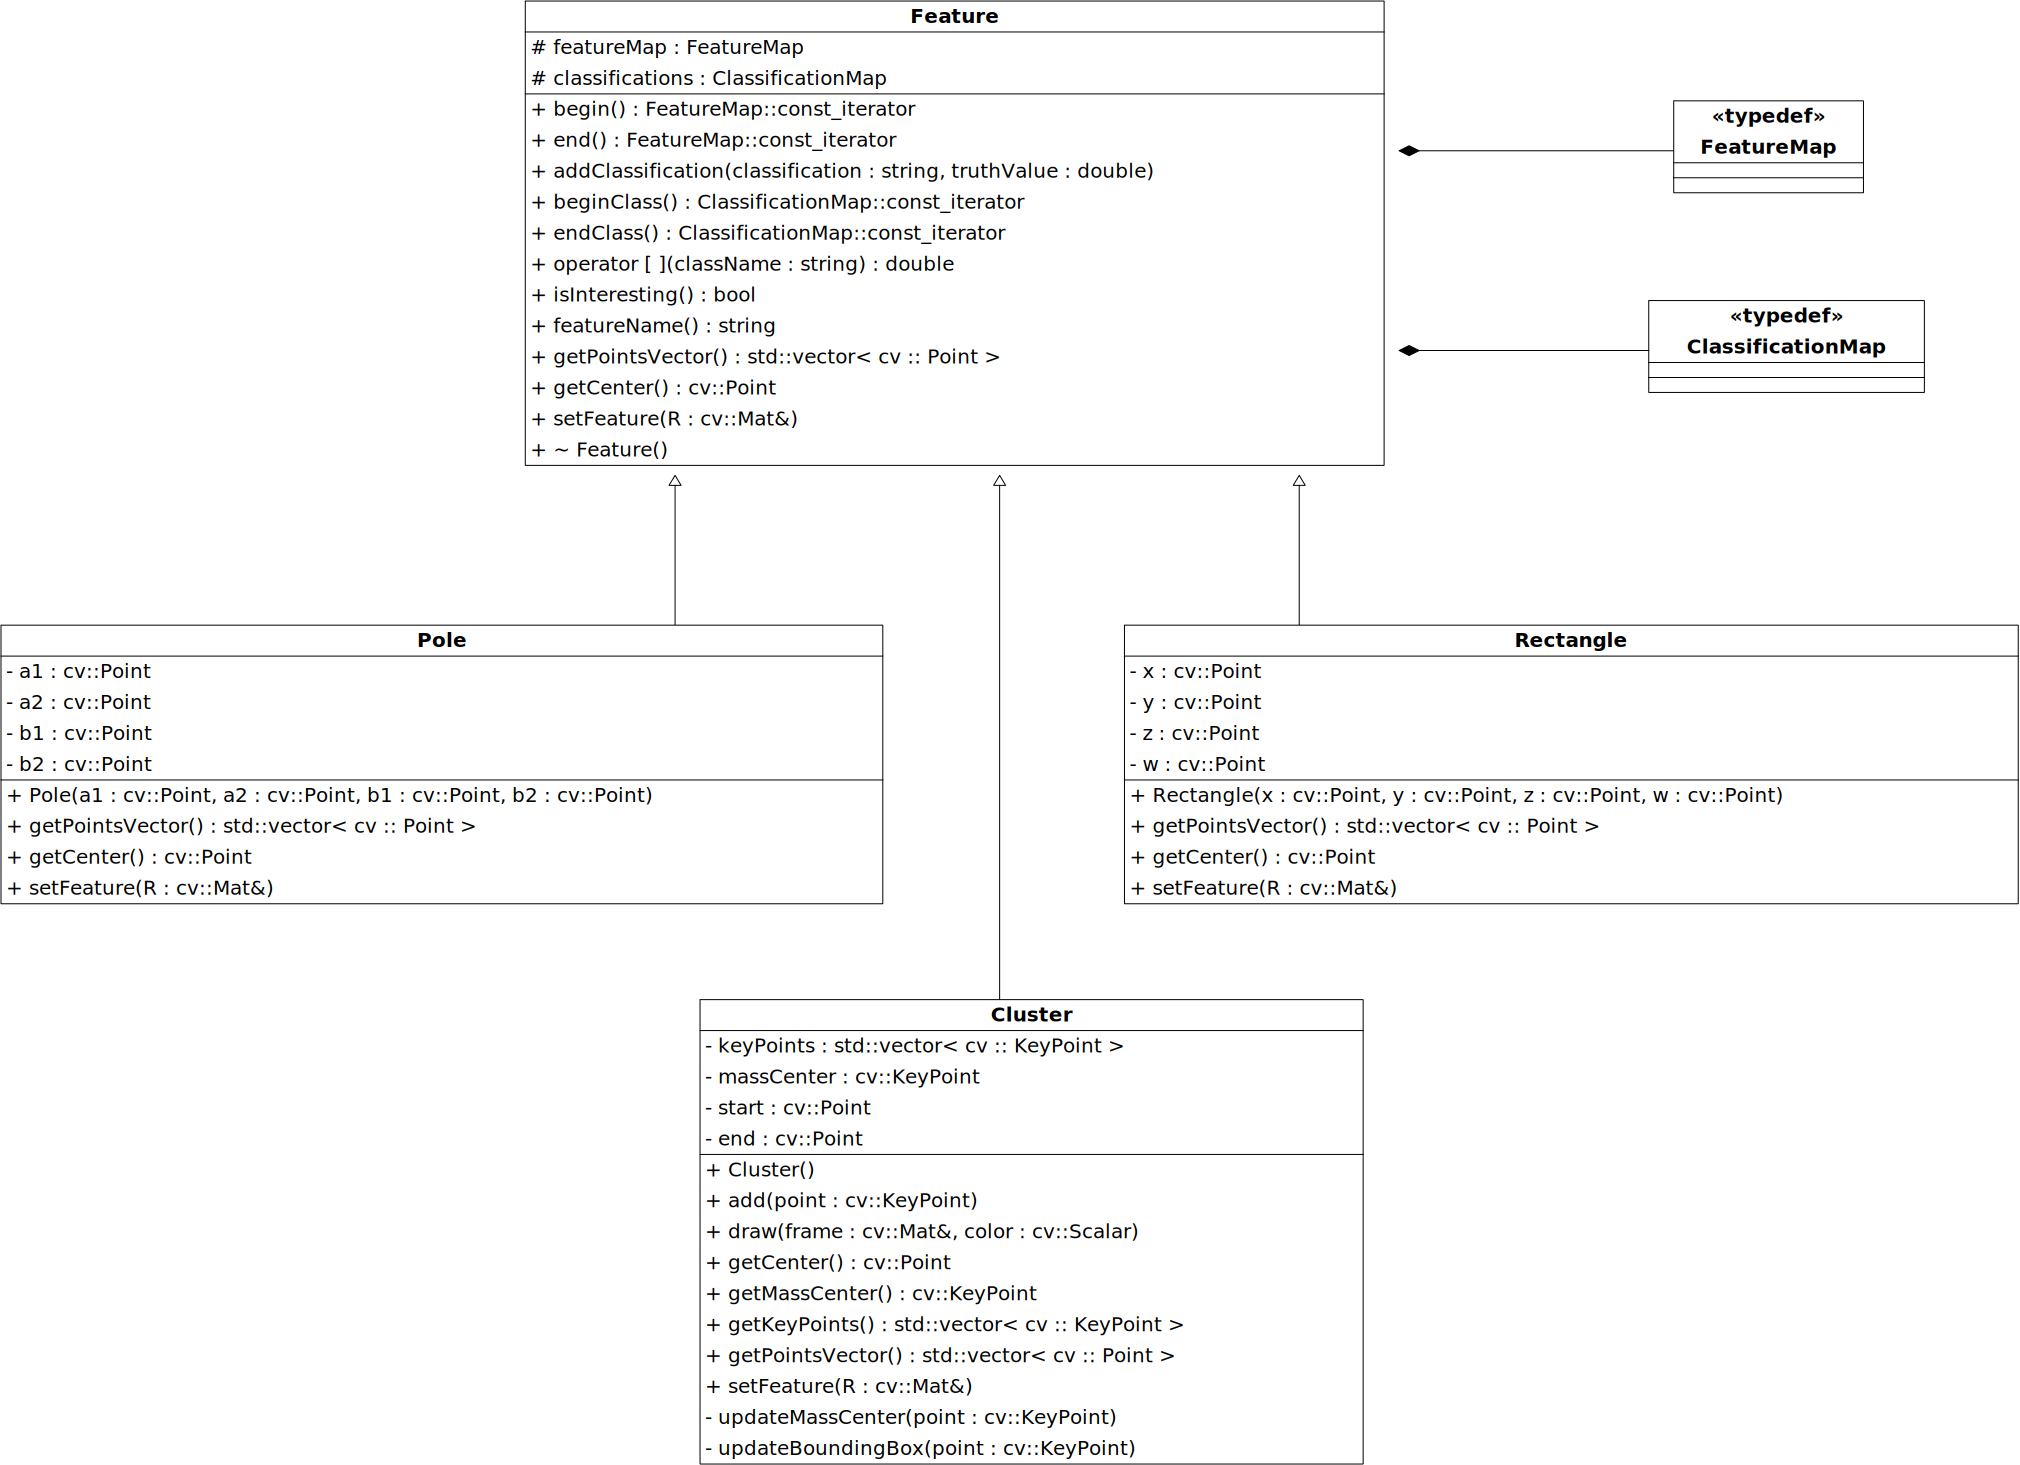
\includegraphics[width=\textwidth]{diagrammi/Feature}
  \caption{Classe Feature e sottoclassi implementate}
  \label{fig:feature}
\end{figure}

Di seguito vengono discussi gli algoritmi implementati per il riconoscimento delle feature geometriche.
La base di partenza per tutti gli algoritmi considerati è l'immagine rettificata della telecamera, ossia l'immagine senza la distorsione causata dalle caratteristiche costruttive della lente, ovvero la distorsione radiale e tangenziale.

\subsection{Quadrilateri}

L'algoritmo di riconoscimento di quadrilateri si basa principalmente sull'algoritmo di Canny~\cite{4767851} per il riconoscimento dei bordi e sulla trasformata di Hough probabilistica~\cite{matas2000robust} per estrarre le linee, o più precisamente, i segmenti, dalla mappa dei bordi.

Le linee estratte contengono, quando l'ambiente è minimamente complesso, molte linee spurie. Inoltre, i quadrilateri interessanti sono composti da due linee approssimativamente orizzontali e due linee approssimativamente verticali. Per questo è stato implementato un algoritmo di filtraggio delle linee in grado di discriminare le linee orizzontali da quelle verticali e dal rumore. Per valutare l'orientamento assoluto delle linee si utilizza la posa del robot. Conoscendo infatti la posa del robot approssimativamente, data l'odometria, è possibile stimare l'inclinazione dell'orizzonte e della linea perpendicolare ad esso. Le linee orizzontali e verticali sono quelle la cui inclinazione, espressa in angolo rispetto all'asse delle ascisse, non supera una determinata soglia rispetto all'orizzonte e alla sua perpendicolare.

Una volta riconosciute le linee verticali e orizzontali viene applicato l'\autorefA{alg:quad-det} per riconoscere quadrilateri e pali.
Viene considerato palo una coppia di linee con un fattore di forma estremamente schiacciato verticalmente. Nell'algoritmo descritto V rappresenta il vettore di linee verticali (ordinate da destra a sinistra), H l'insieme delle linee orizzontali, Q l'insieme di quadrilateri trovati.

\begin{algorithm}[ht]
\caption{QuadrilateralDetector}
\label{alg:quad-det}
\begin{algorithmic}[1] 
\For{$i \in \lbrace 0, VerticalLinesNumber -1 \rbrace$}
  \State $v_{1} \leftarrow V[i]$
  \State $v_{2} \leftarrow V[i+1]$
  \If{$v_{1}$ and $v_{2}$ are not poles}
    \ForAll{$(h_{1},h_{2}) \in H \times H$}
      \State $x \leftarrow$ findInterception($h_{1}$, $v_{1}$);
      \State $y \leftarrow$ findInterception($h_{1}$, $v_{2}$);
      \State $z \leftarrow$ findInterception($h_{2}$, $v_{2}$);
      \State $w \leftarrow$ findInterception($h_{2}$, $v_{1}$);
      \If{$x,y,z,w$ are the vertices of a quadrilateral $q$}
	\State $Q = Q \cup \lbrace q \rbrace$
      \EndIf
    \EndFor
  \EndIf
\EndFor
\Return Q
\end{algorithmic}
\end{algorithm}

Questo algoritmo si basa su una considerazione fondamentale per ridurre la complessità del calcolo, ossia che è altamente probabile che un rettangolo interessante si trovi tra due linee verticali consecutive. Questa considerazione è sostenuta dal fattore di forma dell'immagine, che è largo, e dal fattore di forma della maggior parte dei quadrilateri interessanti, che solitamente sono più stretti che larghi. Questa considerazione non si può tuttavia estendere al caso delle linee orizzontali, per le motivazioni opposte, e per questo la ricerca è fatta in maniera esaustiva.


Per discriminare se un insieme di punti formano o meno un quadrilatero vengono utilizzate due euristiche, a seconda del riconoscimento effettuato.
L'euristica più semplice consiste nel considerare tutto ciò che non è un palo come un quadrilatero. Questa euristica in generale è pessima, ma funziona molto bene, avendo un tasso di recupero decisamente alto, quando il riconoscimento è localizzato.

L'altra euristica possibile che abbiamo sviluppato consiste nello sfruttare le proprietà delle combinazioni convesse. Una combinazione convessa è definita come una combinazione lineare con coefficienti positivi e la cui somma vale 1. L'insieme delle combinazioni convesse di un insieme di punti generano l'involucro convesso dell'insieme.
Nel nostro caso, preso un segmento riconosciuto come possibile lato del quadrilatero, possiamo calcolare qualsiasi punto al suo interno tramite la formula:

\begin{equation}
  x = \alpha\cdot a + (1 - \alpha)\cdot b = b + \alpha\cdot(a - b)
\end{equation}

Dove $a$ e $b$ sono gli estremi del segmento e $x$ è un punto al suo interno, i coefficienti di combinazione convessa sono $\alpha$ e $1 - \alpha$.
Come si nota dalla formula $\alpha = 0$ se $x \equiv b$ e $\alpha = 1$ se $x \equiv a$.
Idealmente, per i vertici di un quadrato, si avrà $\alpha=1$ o $\alpha=0$ se si calcola il coefficiente del vertice rispetto ai due segmenti adiacenti.

Se si prova a calcolare il valore di $\alpha$ con la stessa formula per un punto fuori dal segmento si ottiene un valore maggiore di uno o minore di zero.

L'euristica proposta si basa sulle considerazioni fatte sopra, supponendo che a causa del rumore e altri fattori, i vertici del quadrato riconosciuto si possano trovare all'interno o all'esterno del segmento. Viene quindi calcolato il valore di combinazione convessa di ciascun vertice e, fissata una soglia, viene riconosciuto come quadrato solo un insieme di segmenti i cui vertici hanno $\alpha=1$ o $\alpha=0$, a meno della soglia.

\subsection{Cluster}

I cluster vengono riconosciuti estraendo i keypoint dall'immagine tramite l'algoritmo FAST~\cite{rosten_2006_machine}.
Un keypoint è un punto notevole dell'immagine. Ogni algoritmo di estrazione di keypoint ha delle politiche differenti, ma generalmente rappresentano possibili angoli nell'immagine, ovvero punti con una particolare conformazione del gradiente dell'intensità dei pixel.

Una volta estratti i keypoint, vengono estratti i cluster interessanti tramite l'algoritmo DBSCAN~\cite{ester1996density}.
DBSCAN è un algoritmo che si basa sulla distanza tra i punti. Due punti vengono considerati vicini se la distanza tra di loro è minore di una determinata soglia. Vengono quindi inseriti in un unico cluster tutti i punti che sono raggiungibili tramite la relazione di vicinanza. Ciò significa che tutti i vicini di un punto sono inseriti nello stesso cluster, e allo stesso modo i vicini dei vicini, ricorsivamente.
I cluster che non hanno abbastanza punti al loro interno vengono scartati e considerati come rumore.

\section{Integrazione con il reasoning}
Una volta riconosciute le feature interessanti, vengono calcolati i descrittori di tali feature. I descrittori delle feature vengono inseriti nella FeatureMap, per poter comunicare la feature riconosciuta al classificatore fuzzy.
Viene effettuata la rotazione delle coordinate in modo da avere i quadrilateri riconosciuti il più possibile orientati verticalmente. Questo facilita il compito del reasoner, in quanto attualmente l'operatore ``on'' supporta solo intervalli semplici e non aree o intervalli generici (si veda \autoref{cap:reasoning}).
Le richieste di classificazione delle feature vengono, per quanto possibile, inviate contemporaneamente al reasoner, in modo da rendere possibile l'analisi delle relazioni tra gli oggetti riconosciuti. Al reasoner viene inviato per ogni feature riconosciuta i rispettivi descrittori contenuti nella FeatureMap e un indice univoco. Viene poi popolata, con i dati provenienti dal reasoner, la ClassificationMap. Questo è reso possibile grazie all'indice che identifica le feature univocamente in una richiesta di reasoning.


\section{Livelli di riconoscimento}
Il riconoscimento degli oggetti non è effettuato tramite una singola analisi dell'immagine, ma viene effettuato su più livelli, sfruttando tutte le informazioni possibili.
I due livelli si possono vedere come il livello di individuazione (l'analisi a basso livello) e quello di riconoscimento (l'analisi ad alto livello). Il primo livello si occupa di trovare feature interessanti nell'immagine (e di darne una prima classificazione), mentre il secondo livello si occupa di analizzare in maniera approfondita le feature riconosciute.

Il riconoscimento di basso livello estrae possibili feature dall'immagine intera, in modo che le feature riconosciute possano essere seguite dal tracker. Poiché è importante escludere i falsi positivi il più possibile, e poiché è più complesso analizzare una intera immagine senza conoscere a priori la posizione degli oggetti interessanti, il riconoscimento di basso livello è molto restrittivo. L'euristica utilizzata per riconoscere i quadrilateri nell'immagine è quella che sfrutta le proprietà della combinazione convessa.
Per rendere la computazione più semplice e rapida, non vengono estratti cluster dall'immagine, e le uniche feature analizzate dal reasoner sono i quadrilateri che rappresentano possibili rettangoli.

Una volta riconosciuti i possibili rettangoli interessanti, gli oggetti vengono quindi seguiti dal tracker. Grazie alle informazioni del tracker, descritte nel \autoref{cap:tracking}, è possibile effettuare un'analisi degli oggetti più localizzata. In questa fase è possibile un'analisi dell'immagine più semplice, e quindi si utilizzano tecniche meno discriminative e più robuste. Usiamo quindi l'euristica più semplice (tutto è un quadrilatero) e estraiamo cluster solo in prossimità della regione di interesse, in modo da risparmiare potenza computazionale sia durante l'estrazione delle feature, sia durante il reasoning, eliminando gli oggetti incorrelati. Dato che, in questa ultima fase sono riconosciute più feature, è possibile analizzare feature complesse come gli oggetti composti da più parti, ad esempio le porte.

\chapter{Tracking}
\label{cap:tracking}
\thispagestyle{empty}

\begin{quotation}
{\footnotesize
\noindent\emph{Marty: Ma allora dove diavolo sono? \\
Doc: La domanda giusta è: 'Quando diavolo sono?'}
\begin{flushright}
Ritorno al Futuro, parte I
\end{flushright}
}
\end{quotation}
\vspace{0.5cm}

\section{Introduzione}

Una volta riconosciute le possibili feature, è necessario seguirle nelle immagini successive della telecamera.
Per farlo, ci siamo basati su un algoritmo presente in letteratura, chiamato Consensus-based Matching and Tracking, CMT~\cite{Nebehay2014WACV}.
L'algoritmo considerato è un algoritmo di tracking a lungo termine. Gli algoritmi di tracking a lungo termine permettono di inseguire oggetti che entrano e escono dal campo visivo della telecamera, e cercano di discriminare anche tra oggetti simili.

Il tracker implementato è in grado non solo di riconoscere gli oggetti nell'immagine, ma è in grado, in parte, di capire se gli oggetti riconosciuti dall'algoritmo descritto nel \autoref{cap:riconoscimento} sono già o meno nella lista ddegli oggetti da seguire.

In questo capitolo spiegheremo brevemente come funziona l'algoritmo CMT utilizzato e come è stato integrato con il riconoscimento di oggetti e con la costruzione della mappa.

\section{CMT}

L'idea base dell'algoritmo è che i keypoint siano un buon modo per scomporre in parti l'oggetto da seguire. Il primo passo consiste quindi nell'estrarre keypoint dal bounding box iniziale, calcolare i relativi descrittori delle feature e salvare tutto in un database. Questa idea è resa possibile dal recente sviluppo di algoritmi veloci ed efficienti per l'estrazione di feature quali~\cite{rosten_2006_machine} e~\cite{6126542}.

Successivamente, per ogni frame, i keypoint presenti nell'iterazione precedente vengono inseguiti tramite il calcolo del flusso ottico~\cite{Lucas:1981:IIR:1623264.1623280} di Lukas-Kanade, nella variante piramidale~\cite{Bouguet00pyramidalimplementation}. Inoltre, vengono estratti keypoint e effettuato il matching con i keypoint presenti nel database. I keypoint di cui è stato effettuato con successo il matching vengono sostituiti a quelli seguiti tramite il flusso ottico, poiché si suppone che siano più stabili, non essendo parte di un processo iterativo di valutazione, soggetto ad errore integrale.

La seconda fase consiste in una procedura di votazione per determinare il centro di massa dell'oggetto.
In primo luogo vengono stimate la scala e la rotazione planare dell'oggetto, calcolando la variazione di scala e di rotazione tra tutte le coppie di keypoint e calcolandone la mediana. In seguito, ogni keypoint vota il centro di massa dell'oggetto utilizzando la sua posizione relativa al centro di massa nel primo frame, opportunamente scalato e ruotato grazie ai due valori precedentemente calcolati.

La terza fase dell'algoritmo consiste nell'eliminazione degli outlier tramite un meccanismo di consenso. I centri di massa votati da ciascun singolo keypoint vengono divisi in cluster in base alla distanza euclidea. Quindi, viene individuato il cluster con il maggior numero di voti. Se il cluster scelto ha un numero sufficiente di keypoint, allora l'oggetto viene considerato come visibile e viene calcolato il centro di massa dell'oggetto, eliminando tutti i voti che non appartengono al cluster.

Infine, il bounding box dell'oggetto viene calcolato applicando la rotazione e la scala calcolate precedentemente ai punti del bounding box iniziale. Questo procedimento è il punto più debole dell'algoritmo, perché il bounding box calcolato non tiene conto dell'omografia che può esserci tra il bounding box iniziale e quello attuale, causata, ad esempio, dalla distorsione prospettica a seguito della nuova posa della telecamera.

La nostra implementazione si discosta dall'implementazione originale, su cui è fortemente basata, solo per la possibilità di specificare un bounding box con una forma arbitraria.

\section{Integrazione con il riconoscimento degli oggetti}

L'algoritmo di tracking deve essere in grado di interagire con il riconoscimento a basso e alto livello degli oggetti. Per ottenere questo risultato abbiamo implementato alcune euristiche per gestire a basso livello e in maniera semplice i possibili conflitti tra l'algoritmo di tracking e il riconoscimento.

In primo luogo, per facilitare sia il tracking dell'oggetto, sia il riconoscimento ad alto livello, quando il tracker considera un nuovo oggetto da seguire inviato dal riconoscimento a basso livello, non utilizza il bounding box esatto riconosciuto, ma questo viene maggiorato, scalandolo, in modo da ottenere due importanti risultati:

\begin{enumerate}
 \item Riuscire a riconoscere in maniera efficiente i keypoint che si trovano sui bordi degli oggetti, che spesso sono i keypoint più significativi, soprattutto negli oggetti planari e uniformi, principali obbiettivi di questa tesi.
 \item Riuscire a compensare parzialmente il problema causato dal cambio di posa della telecamera, che potrebbe causare la fuoriuscita dell'oggetto, o parte di esso, dal bounding box, a causa della deformazione prospettica, non calcolata dall'algoritmo.
\end{enumerate}

Le track inviate al riconoscimento di alto livello comprendono due informazioni: il bounding box (maggiorato) e la regione di interesse rettangolare che lo contiene. Questo permette al riconoscimento di alto livello di analizzare solo le regioni di interesse rettangolari dell'immagine, rendendo il compito meno oneroso computazionalmente e di cancellare eventuali feature esterne all'oggetto, che non sono di interesse per il riconoscimento.

L'ultimo problema riguardante l'integrazione, il più problematico, è riuscire a discriminare quali oggetti riconosciuti sono già presenti nella lista delle track.

Questo problema può essere risolto a due livelli. Ad alto livello, è possibile capire che due oggetti tracciati nella mappa occupano lo stesso spazio, e quindi sono lo stesso oggetto. Questa è la soluzione ottimale, ma richiede un grande numero di informazioni e ha un costo computazionale elevato. 
Tuttavia è possibile affrontare a basso livello il problema, almeno parzialmente, escludendo in maniera semplice gli oggetti riconosciuti, con una euristica che abbiamo sviluppato. 
Questa si basa sul calcolo della posizione del centro di massa degli oggetti riconosciuti e delle track, rispetto ai loro bounding box.
Se un oggetto riconosciuto ha il suo centro di massa all'interno di un bounding box di una track attiva, o, viceversa, se una track attiva ha il suo centro di massa nel bounding box dell'oggetto riconosciuto, tale oggetto è considerato già seguito, e non viene aggiunto alla lista delle track.

\begin{figure}[ht]
  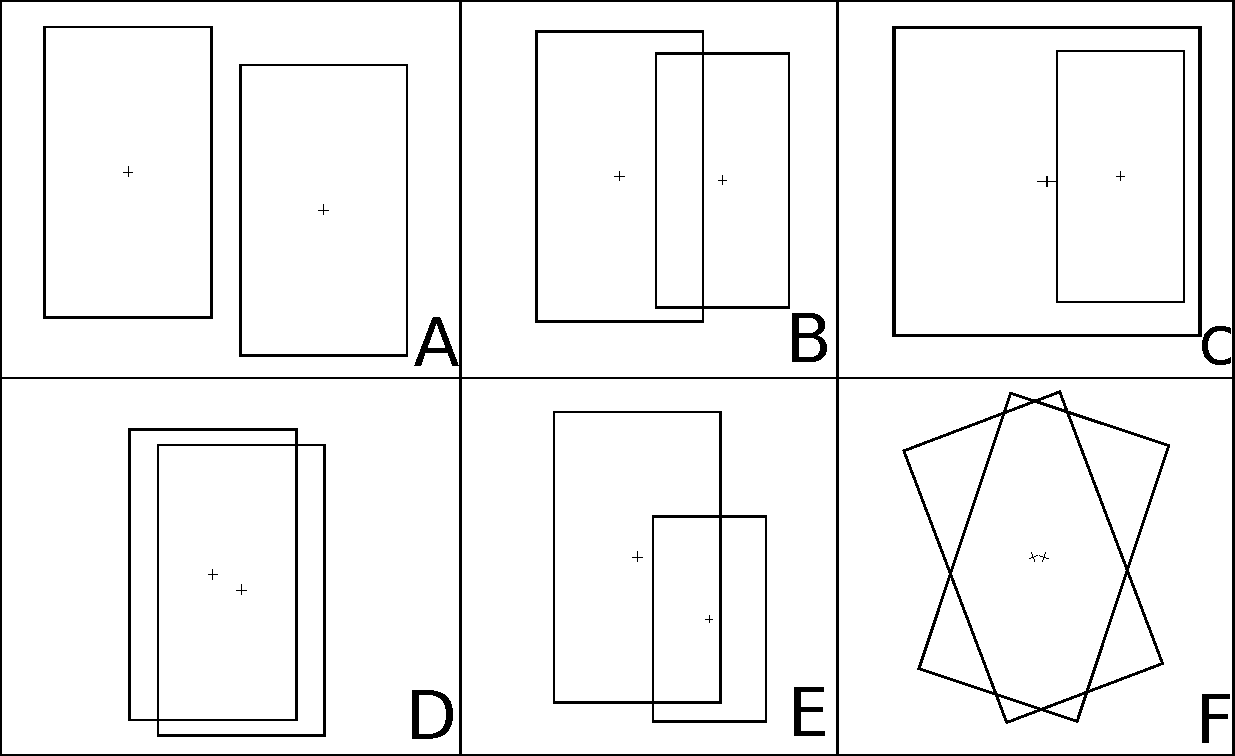
\includegraphics[width=\textwidth]{diagrammi/Euristica}
  \caption[Euristica del tracker]{I possibili posizionamenti delle due track: A. due oggetti differenti e distanti, B. due oggetti differenti abbastanza vicini, con parte del bounding box in comune, C. un oggetto contenente o con di fronte un altro oggetto, D. e F. lo stesso oggetto con due bounding box differenti, E. due oggetti differenti sovrapposti, lo stesso oggetto individuato male oppure un oggetto con una sua parte}
  \label{fig:euristica}
\end{figure}

Come si può vedere dalla \autoref{fig:euristica}, l'euristica copre abbastanza bene quasi tutti i casi, a parte quando si tratta di oggetti composti da più oggetti, o di oggetti che si trovano di fronte ad altri oggetti. Per questi casi sono necessari due ragionamenti ad alto livello differenti: riuscire a capire che un oggetto è semanticamente composto da alcune parti; riuscire a capire che i due oggetti non occupano lo stesso spazio. Per entrambi i ragionamenti non bastano le informazioni estratte dalla singola immagine.

\section{Integrazione con la mappa}
L'euristica descritta nel paragrafo precedente dimostra di comportarsi molto bene nelle situazioni reali, tuttavia subentrano alcuni problemi quando il tracking degli oggetti presenta dei mancati riconoscimenti. Questo causa spesso la sovrapposizione di più track dello stesso oggetto. Questo problema si può risolvere solamente integrando l'algoritmo di tracking con la mappa degli oggetti riconosciuti. Tramite la mappa è facile accorgersi che lo stesso oggetto è seguito più volte, poiché occupa la stessa posizione assoluta dell'oggetto seguito in precedenza.

Il tracking degli oggetti è un compito abbastanza oneroso computazionalmente. Se la posizione del robot è nota, anche in maniera imprecisa, non è necessario mantenere attivo l'algoritmo di tracking per tutti gli oggetti. Inoltre, l'algoritmo usato è soggetto a falsi positivi; potendo filtrare le track che non possono essere attive, perché non si trovano nell'area vista dal robot in un determinato istante, il tasso di falsi positivi cala drasticamente.

Infine, grazie alla stima della posizione, si può calcolare l'omografia che tiene conto della deformazione prospettica del bounding box dell'oggetto rispetto al nuovo punto di vista. Così facendo si può facilitare il riconoscimento ad alto livello.

\chapter{Mapping}
\label{cap:mapping}
\thispagestyle{empty}

\begin{quotation}
{\footnotesize
\noindent\emph{Doc: (leggendo) Ho sepolto la DeLorean nella miniera abbandonata di Delgado accanto al vecchio cimitero dei pistoleros mancati come indicato nell'acclusa mappa. Auspicabilmente dovrebbe restare lì indisturbata finché tu non la riporterai alla luce nel 1955. All'interno troverai le istruzioni per ripararla. Il mio alter-ego del 1955 - e cioè io - non dovrebbe avere problemi a ripararla, così tu potrai ritornare al futuro. Quando sarai tornato nel 1985 distruggi la macchina del tempo. Distruggerla? \\
Marty: Sì, beh, è una storia lunga, Doc!}
\begin{flushright}
Ritorno al Futuro, parte III
\end{flushright}
}
\end{quotation}
\vspace{0.5cm}

\section{Introduzione}
Per risolvere il problema della costruzione della mappa si è deciso di utilizzare un approccio basato sulla fusione multisensoriale. Abbiamo deciso di basare l'implementazione del sistema di localizzazione sulla libreria ROAMFREE, Robust Odometry Applying Multisensor Fusion to Reduce Estimation Errors~\cite{conf/icinco/CucciM13}.
Questa libreria gestisce nativamente una grande varietà di sensori, tra cui la IMU e il magnetometro, e si occupa di integrare questi dati per ottenere una odometria robusta. Inoltre, la libreria permette di integrare sistemi di estrazione di feature, anche differenti e di stimare la posizione degli oggetti considerati.

Il nostro algoritmo utilizza gli oggetti riconosciuti come punti di rifermento nella mappa e localizza il robot rispetto ad essi. 
Per ottenere questo risultato, seguiamo un approccio Full SLAM: viene tenuta traccia di un serie di pose della videocamera e dei punti di riferimento riconosciuti. Da ogni posa del robot è possibile inquadrare un determinato numero di punti di riferimento. Una volta aggiunti una serie di pose e una serie di punti di riferimento, viene ottimizzato simultaneamente l'insieme di pose e la posizione dei punti di riferimento nella mappa, utilizzando il metodo di Gauss-Newton.

Descriveremo nel seguito i dettagli dell'algoritmo utilizzato. Si veda l'\autoref{app:concetti} per i concetti fondamentali necessari alla comprensione dei prossimi paragrafi.


\section{Modello di errore}
Per poter stimare la posizione dei punti di riferimento è necessario definire una misura dell'errore dell'osservazione degli stessi da parte del sistema di estrazione di feature. Il modello usato, trattandosi di una telecamera monoculare, si basa sull'errore di riproiezione della feature nell'immagine.

Abbiamo definito due modelli di errore: uno per analizzare i dati provenienti dal tracker, e un altro per analizzare i dati provenienti dal riconoscimento ad alto livello.

\subsection{Errore sulle track}
Calcoliamo l'errore sulle track come l'errore di riproiezione del centro di massa della track nell'immagine.
Definiamo la previsione della posizione del centro di massa della track $\hat{z}$ nel seguente modo:

\begin{equation*}
 \hat{z} = \colvec{3}{x}{y}{w} = P\colvec{4}{X}{Y}{Z}{W}
\end{equation*}

Definiamo $\hat{z}'$ come:

\begin{equation*}
 \hat{z}' = \colvec{3}{x/w}{y/w}{1}
\end{equation*}

Sia inoltre $z$ l'osservazione proveniente dal tracker del centro di massa della track considerata, definita come:

\begin{equation*}
 z = \colvec{3}{x_{img}}{y_{img}}{1}
\end{equation*}

Definiamo l'errore di riproiezione come:

\begin{equation*}
 e = \hat{z}' - z + \eta
\end{equation*}

Dove $\eta$ è un rumore bianco gaussiano a media nulla.
La metrica utilizzata per minimizzare l'errore di predizione è l'errore quadratico.

\subsection{Errore sugli oggetti}
La funzione di errore sugli oggetti è più complessa, questo perché deve tenere traccia delle informazioni semantiche note dell'oggetto, nel nostro caso la forma.

Poiché l'oggetto è formato da un insieme di punti che definiscono la sua forma, definiamo un sistema di coordinate specifico per ciascun oggetto, e chiamiamo $H$ l'isometria che mappa i punti dell'oggetto nei punti dello spazio a tre dimensioni; $H$ definisce quindi la posa dell'oggetto rispetto allo spazio.
Definiamo dunque ogni punto dell'oggetto nel sistema di coordinate dell'oggetto stesso, in modo da poter gestire in maniera semplice le informazioni metriche provenienti dal riconoscimento.
Definiamo la previsione della posizione dell' i-esimo punto dell'oggetto $\hat{z}_i$ nel seguente modo:

\begin{equation*}
 \hat{z}_i =  P\cdot H\cdot\colvec{4}{X}{Y}{Z}{W}
\end{equation*}

Definiamo come nel caso precedente $\hat{z}'$:

\begin{equation*}
 \hat{z}' = \colvec{3}{x/w}{y/w}{1}
\end{equation*}

l'osservazione dell'i-esimo $z_i$ punto è definita come nel caso precedente:

\begin{equation*}
 z = \colvec{3}{x_{img}}{y_{img}}{1}
\end{equation*}

Definiamo l'errore di riproiezione dell'i-esimo punto come:

\begin{equation*}
 e_i = \hat{z}'_i - z_i + \eta
\end{equation*}

Anche in questo caso la metrica utilizzata per minimizzare l'errore di predizione è l'errore quadratico.

\section{Stima}

\begin{figure}[ht]
  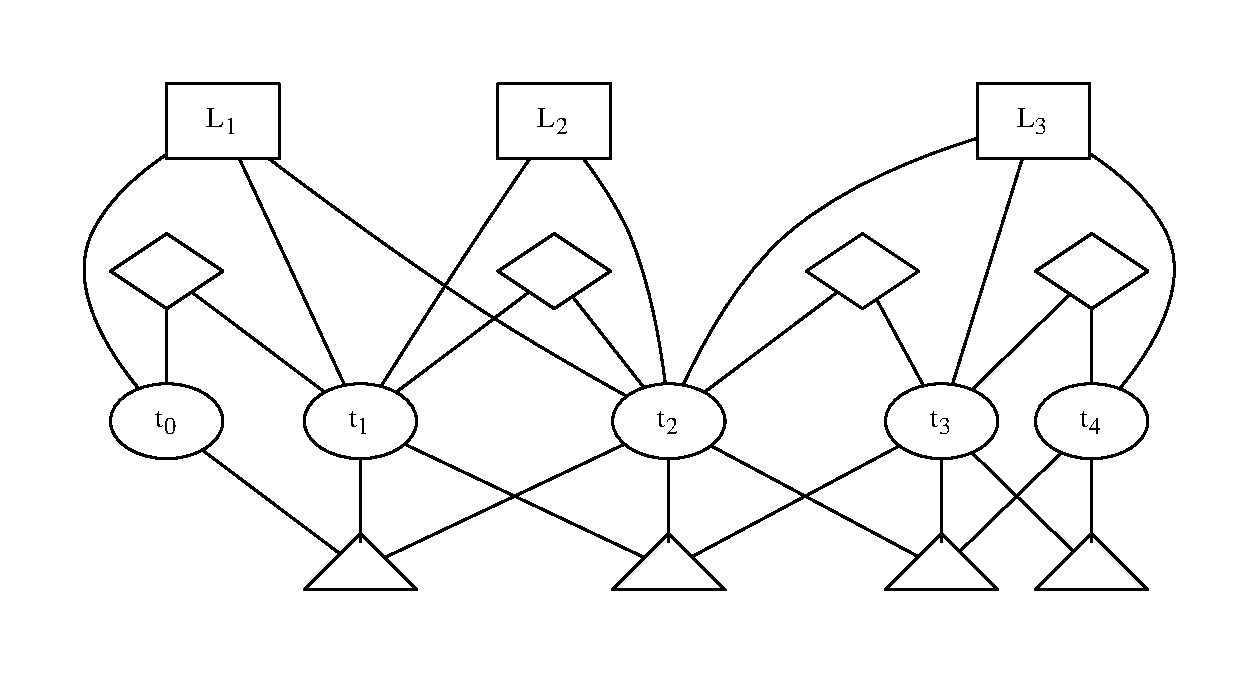
\includegraphics[width=\textwidth]{diagrammi/FactorGraph}
  \caption[Esempio di Factor Graph]{Esempio di un factor graph con nodi che rappresentano le pose (cerchi), e archi che rappresentano i dati della IMU (triangoli) e del magnetometro (rombi). Inoltre sono presenti archi rappresentanti i punti di riferimento (quadrati) }
  \label{fig:FactorGraph}
\end{figure}

La stima delle pose della telecamera e della posizione degli oggetti viene fatta tramite un algoritmo batch di bundle adjustment.
Questo algoritmo si basa su tecniche di inferenza Bayesiane, non lineari, sui factor graph che rappresentano la probabilità congiunta delle variabili di stato, date le misure dei sensori e le feature riconosciute.
Il factor graph è un ipergrafo, in cui ogni nodo rappresenta una possibile posa, mentre ogni arco rappresenta un vincolo di misurazione tra due o più ipernodi. Un esempio di factor graph per questo problema è descritto in \autoref{fig:FactorGraph}.

Per calcolare la stima dei parametri, viene utilizzato lo stimatore di massima verosimiglianza. Sia $\Sigma$ la matrice di covarianza dell'errore e sia $\Omega = \Sigma^{-1}$; il logaritmo della verosimiglianza della misura viene calcolato nel seguente modo:
\begin{equation*}
 \log\mathcal{L}=\sum e^{T}\Omega^{-1}e
\end{equation*}

Utilizziamo il logaritmo della verosimiglianza anziché la verosimiglianza della misura a causa dell'espressione più semplice e facile da massimizzare rispetto alla verosimiglianza, ricordando che applicando una funzione monotona, il valore che massimizza la funzione non varia.
Si utilizza quindi un algoritmo di ottimizzazione basato sul metodo di Gauss-Newton per trovare l'ottimo della distribuzione di probabilità rappresentata dal factor graph, ovvero la configurazione di tutte le variabili di stato che massimizzano la loro probabilità congiunta, date tutte le misure dei sensori e dei punti di riferimento.

Nel caso più semplice, ossia con la sola informazione proveniente dalle track, Le variabili di stato da stimare sono rappresentate semplicemente dal centro di massa delle track, ossia dal centro di massa dei possibili oggetti riconosciuti, e dalla posa della telecamera in ogni istante considerato.

Nel caso di oggetti, le variabili di stato da stimare sono più complesse. Infatti è necessario stimare non solo la posizione relativa dei punti nell'oggetto, ma anche la posa dello stesso, rappresentata dalla matrice $H$; oltre alle pose della telecamera in ogni istante di tempo considerato.



\chapter{Risultati sperimentali}
\label{cap:risultati}
\thispagestyle{empty}

\begin{quotation}
{\footnotesize
\noindent\emph{Doc: Mani in alto! \\
Macchinista: E' una rapina? \\
Doc: E' un esperimento scientifico! Fermi il treno prima di arrivare al prossimo scambio!}
\begin{flushright}
Ritorno al Futuro, parte III
\end{flushright}
}
\end{quotation}
\vspace{0.5cm}

In questo capitolo descriveremo qualitativamente i risultati sperimentali riguardanti i vari moduli del sistema.

\section{Riconoscimento degli oggetti}
Il riconoscimento degli oggetti è abbastanza robusto rispetto ai falsi positivi, a patto che si utilizzi una knowledge base adatta all'ambiente utilizzato. Il riconoscimento è abbastanza robusto rispetto al rumore presente nell'immagine, il sistema ottenuto quindi è abbastanza preciso. 
Tuttavia, il riconoscimento è fortemente basato sugli output dell'algoritmo di Canny per estrarre i bordi e della trasformata di Hough per le linee. In particolare l'algoritmo di Canny è abbastanza sensibile alle variazioni di luce, ed è possibile non riuscire a estrarre correttamente i bordi dall'immagine, e conseguentemente le linee, se le condizioni di luce sono particolarmente sfavorevoli. Questo problema, unito al fatto che la trasformata di Hough probabilistica non riconosce completamente le linee se il bordo riconosciuto da Canny non è abbastanza pulito, fa sì che il tasso di recupero dell'algoritmo non sia elevatissimo. Questo problema è mitigato dall'uso di euristiche meno restrittive e da una analisi localizzata dell'immagine nell'algoritmo di riconoscimento, ma in alcuni casi potrebbe essere problematico nell'algoritmo di individuazione. 

Un'altra possibile causa di cattiva interpretazione dell'immagine è la deformazione prospettica degli oggetti. Infatti, gli oggetti visti da punti di vista particolarmente angolati sono riconosciuti con un fattore di forma molto più schiacciato rispetto alla realtà, e questo può causare una cattiva interpretazione da parte del reasoner. Si può facilmente eliminare il problema calcolando il vero fattore di forma dell'oggetto visto, supponendo che sia un rettangolo, riconducendosi a una rettificazione metrica. Tuttavia questo processo può essere computazionalmente costoso, e in generale non ci è sembrato necessario al fine di implementare un primo prototipo del sistema.

\begin{figure}[ht]
  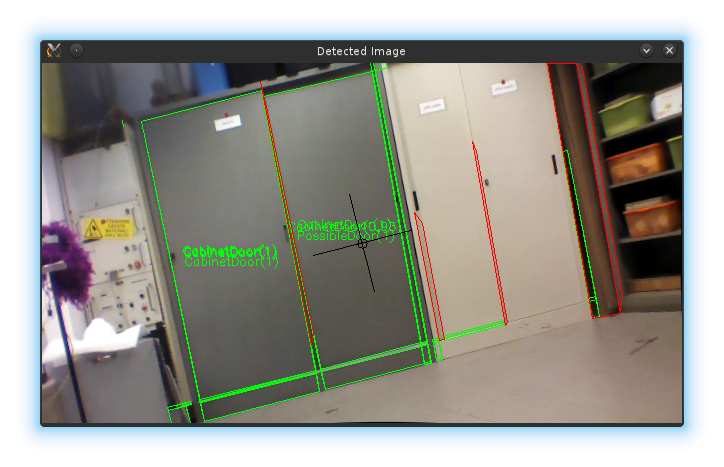
\includegraphics[width=\textwidth]{immagini/risultati/detection}
  \caption[Individuazione degli oggetti]{Individuate le porte dell'armadio}
  \label{fig:detection}
\end{figure}

\begin{figure}[ht]
  \centering
  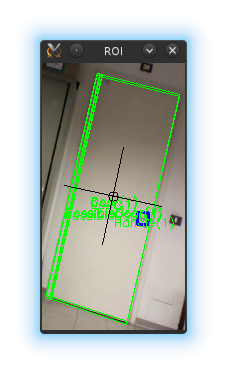
\includegraphics{immagini/risultati/recognition1}
  \caption[Riconoscimento della porta]{Riconosciuta una porta con la sua maniglia}
  \label{fig:recognition1}
\end{figure}

\begin{figure}[ht]
  \centering
  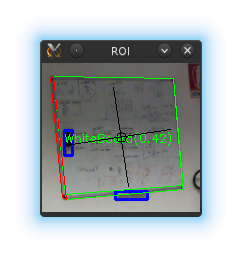
\includegraphics{immagini/risultati/recognition2}
  \caption[Riconoscimento della lavagna]{Riconosciuta la lavagna}
  \label{fig:recognition2}
\end{figure}

\clearpage

\section{Reasoning}
L'algoritmo di reasoning è fortemente dipendente dalla knowledge base implementata. Grazie alla logica fuzzy, se istruito con una knowledge base adatta al contesto, risulta estremamente efficiente e robusto al rumore. Il costo computazionale è estremamente variabile, dipende infatti dal classificatore utilizzato, e dal numero delle istanze da classificare. Se il numero delle istanze è basso, il classificatore riesce a calcolare l'output in tempi dell'ordine di grandezza del millisecondo, su un processore Intel Core i7-4500U.
Se si ha un elevato numero di istanze e si devono gestire relazioni complesse, il tempo di calcolo può essere nell'ordine delle centinaia di millisecondi, o più, se il numero di istanze fosse maggiore a quelle normalmente considerate nei nostri test (nell'ordine delle decine o centinaia).
In generale, il problema dell'algoritmo di reasoning è la natura combinatoria dell'algoritmo utilizzato per risolvere le dipendenze cicliche, in cui è necessario testare ogni possibile combinazione di candidati delle classi considerate. Questo problema può essere risolto in vari modi: 
\begin{itemize}
 \item Restringendo il numero di istanze da classificare simultaneamente a priori, passando solo le istanze correlate all'algoritmo di reasoning.
 \item Scrivendo classificatori intelligenti, in grado di discriminare feature su più livelli della gerarchia, riducendo il numero di candidati che appartengono alle classi coinvolte nelle dipendenze cicliche.
 \item Implementando all'interno del reasoner degli indici di feature basati sui descrittori coinvolti nelle relazioni cicliche, in modo da poter compiere una ricerca basata sul loro valore.
\end{itemize}
Ci è sembrato che le prime due soluzioni fossero più pratiche e semplici da seguire, e quindi le abbiamo implementate nel nostro sistema, lasciando a futuri sviluppi la proposta dell'indicizzazione.

\clearpage

\section{Tracking}
L'algoritmo di tracking usato ha prestazioni estremamente buone. Il tasso di recupero dell'algoritmo è maggiore del 90\%, anche se questo dipende parzialmente dalle caratteristiche dell'oggetto seguito. Il bounding box disegnato non è tuttavia sempre e comunque preciso, soprattutto quando si tratta di seguire oggetti da posizione angolate, dove la deformazione prospettica diventa più significativa. Maggiorando il bounding box, tuttavia, si ottengono risultati buoni anche quando il punto di vista è moderatamente angolato, poiché l'oggetto risulta essere contenuto completamente nel bounding box considerato.

La precisione dell'algoritmo non è altrettanto buona, poiché si possono verificare riconoscimenti errati, soprattutto quando l'oggetto considerato non è nel campo visivo della telecamera. Infatti, poiché l'algoritmo considera una sola istanza possibile dell'oggetto considerato, sarà il vero oggetto a essere riconosciuto.

Per quanto riguarda il costo computazionale, l'algoritmo riesce a lavorare ad elevato frame rate se gli oggetti seguiti simultaneamente sono pochi. Questo quindi può essere un problema quando si devono costruire mappe con molti oggetti. Il problema tuttavia è risolto in maniera abbastanza semplice considerando come track attive solo quelle che potrebbero trovarsi nel campo visivo del robot, anziché tutte le track seguite, ed eventualmente limitando il numero di match cercati nell'immagine a ogni iterazione. Utilizzando la mappa si risolve anche quasi totalmente il problema del riconoscimento errato delle track fuori dall'immagine.
L'ultimo aspetto da considerare dell'algoritmo di tracking implementato è la sua capacità di riconoscere un oggetto già seguito.
Abbiamo notato che l'euristica da noi implementata funziona estremamente bene nella maggior parte dei casi, soffrendo solo qualche problema quando l'algoritmo di tracking, a causa del numero elevato di track, non riesce ad avere un frame rate paragonabile al nodo che individua gli oggetti. In questi casi, l'algoritmo di tracking potrebbe non aver riconosciuto in tempo un oggetto entrato nell'immagine, che invece è stato già individuato, generando una nuova track sull'oggetto. Questo problema tuttavia può essere facilmente risolto a livello di mappa, riuscendo a individuare gli oggetti che occupano lo stesso spazio come equivalenti.

\begin{figure}[ht]
  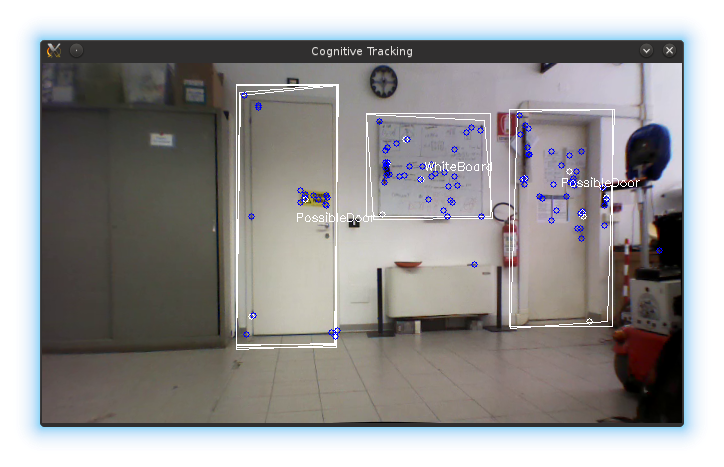
\includegraphics[width=\textwidth]{immagini/risultati/tracker1}
  \caption{L'algoritmo di riconoscimento ha individuato la lavagna due porte}
  \label{fig:tracker1}
\end{figure}

\begin{figure}[ht]
  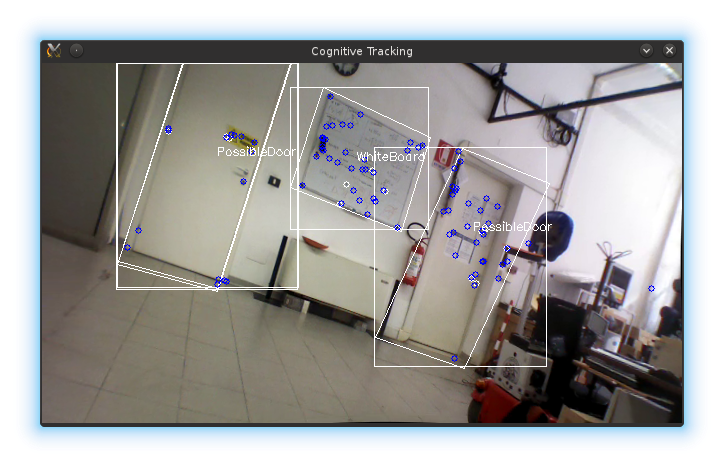
\includegraphics[width=\textwidth]{immagini/risultati/tracker2}
  \caption{Il tracker insegue gli oggetti precedentemente riconosciuti}
  \label{fig:tracker2}
\end{figure}
\chapter{Conclusioni e Sviluppi Futuri}
\label{cap:sviluppi}
\thispagestyle{empty}

\begin{quotation}
{\footnotesize
\noindent\emph{Jennifer: Avevo portato questo bigliettino dal futuro e ora si è cancellato! \\
Doc: Certo che si è cancellato! \\
Jennifer: Ma che cosa significa? \\
Doc: Significa che il vostro futuro non è ancora stato scritto, quello di nessuno. Il vostro futuro è come ve lo creerete. Perciò createvelo buono, tutti e due. \\
Marty: Lo faremo, Doc!}
\begin{flushright}
Ritorno al Futuro, parte III
\end{flushright}
}
\end{quotation}
\vspace{0.5cm}

In questa tesi abbiamo dimostrato che è possibile sviluppare un sistema SLAM che sia basato sul riconoscimento degli oggetti, anziché su feature geometriche di basso livello come angoli e linee. Abbiamo inoltre dimostrato che non è necessario utilizzare procedure di apprendimento dispendiose e grandi dataset per riconoscere oggetti, ma è sufficiente riuscire a estrarre abbastanza informazione per dare una descrizione concettuale dell'oggetto, tramite formule logiche; tutto questo mantenendo limitato il numero di risorse computazionali richieste.
Riconoscere oggetti invece che feature di basso livello ha molti grossi vantaggi:
\begin{itemize}
 \item In generale, non vengono confusi l'uno con l'altro, questo rende più semplice implementare algoritmi di chiusura dei cicli.
 \item Contengono molta più informazione che può essere sfruttata rispetto alle feature geometriche di basso livello, questo permette di avere molti vincoli sulla posizione dei punti nello spazio.
 \item Permettono di compiere ragionamenti semantici: 
  \begin{itemize}
   \item \`E possibile capire il tipo di stanza in cui ci si trova.
   \item \`E possibile adattarsi ai cambiamenti di apparenza o forma degli oggetti, ad esempio una porta che si apre.
   \item \`E possibile inferire ulteriore informazione, come ad esempio la presenza di una parete sullo stesso piano di una porta.
   \item \`E possibile impostare politiche di navigazione semantiche, impostare politiche ad hoc a seconda della vicinanza a specifici oggetti.
  \end{itemize}
\end{itemize}

Uno dei contributi più significativi della tesi è lo sviluppo di un nuovo modello di classificatore ad albero. Il corrente stato dell'arte sugli alberi di decisione e sugli alberi di decisione fuzzy non prende in considerazione le eventuali relazioni semantiche tra gli oggetti in input al classificatore, non permettendo di sfruttare le relazioni tra gli oggetti per rendere più robusta la classificazione.
Abbiamo definito alcune possibili relazioni tra gli oggetti, e un algoritmo di reasoning in grado di sfruttarle. Abbiamo anche considerato oggetti che sono definiti solo in base alla loro reciproca relazione e risolto il problema della loro classificazione.

Abbiamo verificato l'utilità degli algoritmi di tracking a lungo termine nel campo della localizzazione, analizzandone vantaggi e svantaggi, e proponendo delle soluzioni per il loro uso pratico, grazie all'integrazione con la mappa costruita.

Questa tesi lascia comunque aperti molti problemi. Possiamo pensare a molte estensioni dell'attuale sistema.

In primo luogo si può pensare di estendere e migliorare il riconoscimento delle feature di basso livello. Un'alternativa interessante potrebbe essere sfruttare le reti neurali convoluzionali per l'estrazione rapida ed efficiente di feature a basso livello come forme e caratteristiche geometriche e usare algoritmi di clustering (k-means, fuzzy c-means) per determinare il colore delle feature. Inoltre, si potrebbe sfruttare le proprietà geometriche degli oggetti per calcolare la rettificazione metrica della feature, ottenendo così una stima migliore del fattore di forma.

Inoltre, si potrebbe estendere il reasoner per aggiungere altri tipi di relazioni tra gli oggetti, in aggiunta a quelle considerate da questa tesi, o estendere la capacità del reasoner di gestire spazi di variabili a più dimensioni.

Infine, si potrebbe pensare di lavorare sugli algoritmi di tracking e localizzazione per aumentare le loro prestazioni, sfruttando le informazioni reciproche per aumentare le prestazioni di riconoscimento e di costo computazionale.

Altri aspetti restano completamente inesplorati, come l'eventuale reasoning concettuale sulla stanza e la rilevazione di altre categorie di oggetti, uno stack di navigazione basato sugli oggetti riconosciuti, il controllo della scala attuale della mappa per discriminare gli oggetti individuati grazie alla loro dimensione. In particolare una volta riconosciuti una classe di oggetti come porte e finestre, dovrebbe essere possibile riconoscere i muri della stanza.


\cleardoublepage
% ---- Bibliography ----
\bibliographystyle{plain}
\pagenumbering{Roman}
\bibliography{altro/bibliografia}

\appendix

\pagestyle{fancy} 
\fancyfoot{}                                               
\renewcommand{\chaptermark}[1]{\markboth{\appendixname\ \thechapter.\ #1}{}} 
\renewcommand{\sectionmark}[1]{\markright{\thesection.\ #1}}         
\fancyhead[LE,RO]{\bfseries\thepage}    
                                        
\fancyhead[RE]{\bfseries\leftmark}    
\fancyhead[LO]{\bfseries\rightmark}     
\renewcommand{\headrulewidth}{0.3pt} 

\chapter{Concetti Fondamentali}
\label{app:concetti}
\thispagestyle{empty}

\begin{quotation}
{\footnotesize
\noindent{\emph{Doc: Ovviamente il continuum temporale è stato interrotto creando questa nuova temporale sequenza di eventi risultanti in questa realtà alternativa. \\
Marty: Che lingua è Doc? \\
Doc: Ah si, si, si, si, si! Lascia che ti spieghi. Immagina, che questa linea rappresenti il tempo\dots}}
\begin{flushright}
Ritorno al Futuro, parte II
\end{flushright}
}
\end{quotation}
\vspace{0.5cm}

Si introducono in questo capitolo di seguito i concetti fondamentali alla comprensione della tesi.

\section{Logica Fuzzy}
La logica fuzzy è una logica multi valore che permette di esprimere non solo la verità o la falsità di una affermazione, ma anche un grado di verità, che può essere qualsiasi numero tra 0 (ossia l'affermazione è falsa) e 1 (ossia l'affermazione è vera). Questa propriet\`a fa della logica fuzzy uno strumento appropriato per modellare aspetti del mondo reale quando si sia in presenza di incertezza.

Tra l'altro, grazie a questa logica è anche possibile esprimere concetti che in una logica a due valori sarebbero paradossali.
Ad esempio, la frase ``sono un bugiardo'', che nella logica a due valori risulta paradossale, nella logica fuzzy può assumere valori consistenti.

\subsection{Insiemi Fuzzy}
La logica fuzzy è basata fortemente sul concetto di insieme fuzzy. Un insieme fuzzy è un insieme la cui funzione di appartenenza può avere valori nell'intervallo $[0, 1]$.
I fuzzy set sono quindi definiti da una funzione di appartenenza $f$ definita su un dominio $D$, avente come codominio l'intervallo $[0,  1]$.  Formalmente un fuzzy et è definito come:

\begin{equation*}
 f:D\rightarrow [0, 1]
\end{equation*}

Si definisce variabile linguistica $X$, definita sulla variabile di base $u$ una tupla così definita:
\begin{equation*}
(X, T(X), U, G, M)
\end{equation*}

dove:

\begin{description}
 \item [X] è il nome della variabile.
 \item [T(X)] è un insieme di termini, detti anche valori linguistici, che costituiscono il dominio di X.
 \item [U] è il dominio della variabile di base $u$.
 \item [G] è una regola sintattica per generare l'interpretazione di X per ogni valore di u.
 \item [M] è una regola semantica che associa a X il suo significato.
\end{description}


Data una variabile $x$, è possibile definire più fuzzy set rispetto al suo dominio. Si parla di frame of cognition quando valgono le seguenti condizioni:
\begin{enumerate}
 \item L'intero dominio della variabile è coperto da almeno un fuzzy set con valore di verità maggiore di zero.
 \item Tutti i fuzzy set sono unimodali.
 \item Tutti i fuzzy set sono normali.
\end{enumerate}

Inoltre si parla di partizione fuzzy, se la somma delle funzioni di appartenenza di ogni fuzzy set in ogni punto del dominio è uguale a 1.

La normale teoria degli insiemi è contenuta nella teoria degli insiemi fuzzy. Infatti, un intervallo è un insieme fuzzy, con valore di verità di tutti gli elementi pari a 1. Anche i singoli elementi possono essere trattati, tramite il fuzzy set singleton, che ha valore di verità 1 per un solo elemento del dominio, e 0 per tutti gli altri.

\subsection{Operazioni sui fuzzy set}

Sui fuzzy set sono definite le seguenti operazioni:
\begin{itemize}
 \item unione
 \item intersezione
 \item complemento
 \item aggregazione
\end{itemize}

\subsubsection{Complemento}

Dato un insieme fuzzy $A$, con funzione di appartenenza $\mu_A$ il complemento è definito come:

\begin{equation*}
 c(\mu_A(x)) = \mu_{\neg A}(x)
\end{equation*}

Il complemento di insiemi fuzzy deve rispettare i seguenti assiomi:
\begin{enumerate}
 \item $c(0)=1$, $c(1)=0$ (condizioni al contorno)
 \item $c$ è una funzione continua.
 \item $c$ è involutiva, ossia $c(c(a))=a\, \, \forall a \in [0, 1]$
\end{enumerate}

l'unica funzione che rispetta i seguenti assiomi è la funzione:

\begin{equation*}
 c(x) = 1 - x
\end{equation*}

\subsubsection{Intersezione}

Dati due insiemi fuzzy $A$ e $B$, con funzione di appartenenza $\mu_A$ e $\mu_B$ l'intersezione  è definita come:

\begin{equation*}
 i(\mu_A(x), \mu_B(x)) = \mu_{A\cap B}(x)
\end{equation*}

L'intersezione di insiemi fuzzy deve rispettare i seguenti assiomi:

\begin{enumerate}
 \item $i(a, 1)=a$ (condizioni al contorno)
 \item $d\geq b \implies  i(a,d)\geq i(a,b)$ (monotonicità)
 \item $i(b,a) = i(a,b)$ (commutatività)
 \item $i(i(a,b),d)=i(a,i(b,d))$ (associatività)
 \item $i$ è una funzione continua
 \item $a\geq i(a,a)$ (sub-idempotenza)
 \item $a_1<a_2 \wedge b_1<b_2\implies i(a_1,b_1)<i(a_2,b_2)$ (monotonicità stretta)
\end{enumerate}

Non esiste un'unica funzione che rispetta questi assiomi. Ogni funzione che rispetta questi assiomi viene detta T-norm.
Esempi di T-norm sono l'operatore minimo e il prodotto tra i valori di verità.

\subsubsection{Unione}

Dati due insiemi fuzzy $A$ e $B$, con funzione di appartenenza $\mu_A$ e $\mu_B$ l'unione è definita come:

\begin{equation*}
 u(\mu_A(x), \mu_B(x)) = \mu_{A\cup B}(x)
\end{equation*}

L'unione di insiemi fuzzy deve rispettare i seguenti assiomi:

\begin{enumerate}
 \item $u(a, 0)=a$ (condizioni al contorno)
 \item $b \leq d \implies u(a,b) \leq u(a,d)$ (monotonicità)
 \item $u(a,b) = u(b,a)$ (commutatività)
 \item $u(a,u(b,d)) = u(u(a,b),d)$ (associatività)
 \item $u$ è una funzione continua
 \item $u(a,a) \geq a$ (super-idempotenza)
 \item $a_1< a_2 \wedge b_1 < b_2 \implies u(a_1,b_1)<u(a_2,b_2)$ (monotonicità stretta)
\end{enumerate}

Non esiste un unica funzione che rispetta questi assiomi. Ogni funzione che rispetta questi assiomi viene detta T-conorm, o S-norm.
Esempi di S-norm sono l'operatore massimo e la somma probabilistica tra i valori di verità.
La somma probabilistica $p$ tra due variabili $a$  e $b$ è definita come:

\begin{equation*}
 p = a+b - a\cdot b 
\end{equation*}

\subsection{Aggregazione}

Dato un insieme di fuzzy set $(A_1, \dots, A_n)$, con funzione di appartenenza $(\mu_{A_1}, \dots, \mu_{A_n})$ l'insieme fuzzy aggregato $A$ è definito come:

\begin{equation*}
   \mu_A(x) = h(\mu_{A_1}(x), \dots, \mu_{A_n}(x))
\end{equation*}

L'aggregazione di fuzzy set deve rispettare i seguenti assiomi:

\begin{enumerate}
 \item $h(0, \dots, 0)=0, h(1, \dots, 1)=1 $ (condizioni al contorno)
 \item $a_i \leq b_i\, \forall i \implies h(a_1, a_n) \leq h(b_1, b_n)$ (monotonicità)
 \item $h$ è una funzione continua
 \item $h(a, \dots,a)=a$ (idempotenza)
 \item $h(a_1,\dots,a_n) = h(a_i, \dots, a_j)\, \forall i,\dots, j\in [1,n]$ (simmetria) %%
\end{enumerate}

Non esiste un unica funzione che rispetta questi assiomi. Un esempio di operatore di aggregazione valido è la media generalizzata:
\begin{equation*}
 h(a_1, \dots, a_n) = \dfrac{(a_1^\alpha + \dots + a_n^\alpha)^{1/\alpha}}{n}
\end{equation*}



\subsection{Regole Fuzzy}

Una regola di inferenza fuzzy può essere considerata come un modello, un mezzo per definire una funzione tra un ingresso e una uscita.

Le regole fuzzy che consideriamo sono composte nel seguente modo:
\begin{verbatim}
 IF <antecedente> THEN <consequente>
\end{verbatim}

Dove l'antecedente è una formula logica ben formata è il conseguente è una o più proposizioni legate dall'operatore and.

Una formula ben formata è definita come:

\begin{itemize}
 \item Una proposizione è una formula ben formata
 \item Se ``A'' è una formula ben formata, anche ``not A'' è una formula ben formata.
 \item Se ``A'' e ``B'' sono formule ben formate anche ``A and B'', ``A or B'' sono formule ben formate.
 \item null'altro è una formula ben formata.
\end{itemize}

Una proposizione è definita come un assegnamento di una etichetta a una variabile fuzzy, del tipo
\begin{verbatim}
 <VARIABLE> IS <LABEL>
\end{verbatim}

esistono due tipi di regole:
\begin{description}
 \item [Regole linguistiche] note anche come regole di Mamdami, dove il conseguente è la congiunzione di più clausole linguistiche. Queste regole possono essere considerate come una funzione che mappa una configurazione di input in ingresso a una interpretazione simbolica dell'output desiderato. 
 \item [Regole di modello] note anche come regole di Takagi-Sugeno-Kosko. In questo tipo di regole le proposizioni nel conseguente sono del tipo: \verb|<VARIABLE> IS f(...)|. Questo tipo di regole legano un modello alla variabile di uscita. La funzione \verb|f| può essere definita in qualunque modo, e prende in input le variabili di base delle variabili linguistiche presenti sul lato sinistro della regola.

\end{description}


Un insieme di regole fuzzy forma una knowledge base. Le regole della knowledge base possono avere diversi pesi, in modo da rendere più importanti alcune regole specifiche, oppure evitare la preponderanza delle regole lunghe rispetto a quelle corte.
L'inferenza sulla knowledge base viene fatta come segue: 

\begin{enumerate}
 \item Dato un insieme di fatti noti, ossia variabili linguistiche di cui si conosce il valore, vengono selezionate solo le regole il cui antecedente contiene solo le variabili note.
 \item Viene calcolato il valore di verità del lato sinistro delle regole
 \item Se specificato, il valore di verità viene combinato con il peso della regola.
 \item Viene aggregato l'output da regole diverse che calcolano la stessa etichetta.
 \item Viene defuzzificato, eventualmente, l'output simbolico calcolato, oppure viene compiuta una approssimazione linguistica, ossia viene calcolata l'etichetta in output che meglio approssima, decisa una metrica, l'output simbolico calcolato (che può contenere più etichette per la stessa variabile)
\end{enumerate}

Esistono vari tipi di defuzzificazione. L'operazione di defuzzificazione viene applicata all'insieme di insiemi fuzzy ricavati per ciascuna variabile linguistica. I metodi più noti sono:
\begin{itemize}
 \item Centro di massa
 \item Bisettrice
 \item Media dei massimi
 \item Minor massimo
 \item Maggior massimo
 \item Centro dell'area più alta
\end{itemize}

Il metodo più usato in assoluto è il centro di massa applicato a singleton.

\section{Geometria della telecamera}

Verrà descritta brevemente la geometria della telecamera.
Una telecamera è un dispositivo in grado di acquisire immagini del mondo. Essa è composta da una lente e un piano dell'immagine, in grado di acquisire l'immagine. Nel nostro modello consideriamo la lente come estremamente sottile, in modo da non considerare le distorsioni radiali e tangenziali dovute alla lente. La lente è necessaria in quanto essa è in grado di convogliare tutta la luce proveniente da un determinato punto dello spazio in un unico punto (oppure in un'area di punti) nel piano immagine.

Chiamiamo asse ottico l'asse perpendicolare al piano dell'immagine passante per il centro della lente. Si chiama Principal Point l'intersezione tra l'asse ottico e il piano dell'immagine.
Chiamiamo distanza focale la distanza tra la lente e il piano dell'immagine.

\subsection{Geometria proiettiva}

La relazione tra le coordinate della telecamera e le coordinate dei punti del mondo è una relazione non lineare.
Dato un punto nello spazio $P=(X,Y,Z)$, la sua proiezione nel piano dell'immagine $p=(x,y)$ avrà le seguenti coordinate:

\begin{equation*}
 \begin{aligned}
  x = f\cdot \dfrac{X}{Z} \\
  y = f\cdot \dfrac{Y}{Z}
 \end{aligned}
\end{equation*}

Con $f$ distanza focale della telecamera.

Per semplificare il problema, viene usato un altro sistema di coordinate in cui la relazione considerata è una relazione lineare.
Queste coordinate sono dette coordinate omogenee, e uno spazio che le utilizza viene detto spazio proiettivo.

Le coordinate omogenee sono delle coordinate che per esprimere uno spazio a $n$ dimensioni, utilizzano $n+1$ coordinate. Le coordinate spaziali sono definite a meno di un fattore moltiplicativo, ovvero $P = \alpha\cdot P$.
La quarta coordinata ha inoltre un significato particolare. Se è diversa zero il punto rappresenta un punto reale dello spazio euclideo, altrimenti rappresenta una direzione, detto anche punto all'infinito.


\subsubsection{Piano immagine}
Modelliamo l'immagine con uno spazio proiettivo a due dimensioni, $\mathcal{P}^2$.
Un punto $X$ del piano immagine è definito come:
\begin{equation*}
  X=\colvec{3}{x}{y}{w}
\end{equation*}

E' possibile anche definire una retta $l$ nel piano immagine sempre utilizzando il vettore tridimensionale:

\begin{equation*}
  l=\colvec{3}{a}{b}{c}
\end{equation*}

Un punto $X$ appartiene a una retta $l$ se:

\begin{equation*}
 X^T\cdot l = 0
\end{equation*}

Equivalentemente si può dire che una retta $l$ passa per un punto $X$ se:

\begin{equation*}
 l^T\cdot X = 0
\end{equation*}

l'equazione di una retta è quindi definita come:

\begin{equation*}
 a\cdot x + b \cdot y+ c \cdot w = 0
\end{equation*}

Anche la retta quindi è definita a meno di un coefficiente moltiplicativo.
La retta che contiene tutti i punti all'infinito è detta linea all'infinito $l_\infty$.

Nello spazio a due dimensioni è estremamente semplice calcolare la retta passante per due punti o il punto intersezione di due rette. Basta usare il prodotto vettoriale tra due elementi. Per calcolare la retta $l$ passante per due punti scriviamo:

\begin{equation*}
 l = P_1 \times P_2
\end{equation*}

Per calcolare il punto di intersezione $P$ tra due rette:

\begin{equation*}
 P = l_1 \times l_2
\end{equation*}


E' possibile esprimere anche coniche nel piano proiettivo. Una conica $C$ è definita come:

\begin{equation*}
 C = \begin{pmatrix} a & b & c \\ b & d & e \\ c & e & f \\ \end{pmatrix}
\end{equation*}

Si può notare che la matrice è simmetrica. Questo avviene senza perdita di generalità.
Un punto appartiene a una conica se:

\begin{equation*}
 X^T\cdot C \cdot X = 0
\end{equation*}

Anche le coniche sono definite a meno di un coefficiente moltiplicativo.

Infine è possibile esprimere coniche duali. Se le coniche sono insieme di punti, le coniche duali sono insieme di linee.
Si può dimostrare che la conica duale $C^*$ alla conica $C$ è:
\begin{equation*}
 C^*=C^{-1}
\end{equation*}

una retta appartiene alla conica duale se:

\begin{equation*}
 l^T\cdot C^* \cdot l = 0
\end{equation*}

Lo spazio proiettivo a 2 dimensioni ha due punti notevoli detti punti circolari. Tutte le possibili circonferenze si intersecano nei punti circolari, che sono due punti immaginari:

\begin{equation*}
 \begin{aligned}
  I=\colvec{3}{1}{i}{0} & & J=\colvec{3}{1}{-i}{0}
 \end{aligned}
\end{equation*}

I punti circolari appartengono a $l_\infty$.

Questi due punti possono essere espressi in maniera compatta dalla conica duale ai punti circolari, una conica degenere, che può essere calcolata come:

\begin{equation*}
 C^*_\infty = I\cdot J^T + J\cdot I^T =\begin{pmatrix} 1 & 0 & 0 \\ 0 & 1 & 0 \\ 0 & 0 & 0 \\ \end{pmatrix}
\end{equation*}


\subsubsection{Mondo reale}
Modelliamo il mondo reale con uno spazio proiettivo a 3 dimensioni, $\mathcal{P}^3$.

Un punto $X$ del mondo reale è definito come:
\begin{equation*}
  X=\colvec{4}{x}{y}{z}{w}
\end{equation*}

E' possibile anche definire piano $\pi$ nel mondo reale utilizzando il vettore quadridimensionale:

\begin{equation*}
  \pi=\colvec{4}{a}{b}{c}{d}
\end{equation*}

Un punto $X$ appartiene a una piano $\pi$ se:

\begin{equation*}
 X^T\cdot \pi = 0
\end{equation*}

Equivalentemente si può dire che un piano $\pi$ passa per un punto $X$ se:

\begin{equation*}
 \pi^T\cdot X = 0
\end{equation*}

l'equazione di un piano è quindi definita come:

\begin{equation*}
 a\cdot x + b \cdot y+ c \cdot z + d \cdot w = 0
\end{equation*}

Anche il piano quindi è definito a meno di un coefficiente moltiplicativo.
Il piano che contiene tutti i punti all'infinito e, conseguentemente, tutti le rette all'infinito di tutti i piani dello spazio, si chiama piano all'infinito $\pi_\infty$. 

E' possibile esprimere anche quadriche nel piano proiettivo. Una quadrica $Q$ è definita come:

\begin{equation*}
 Q = \begin{pmatrix} a & b & c & d \\ b & e & f & g \\ c & f & h & i \\ d & g & i & l \\ \end{pmatrix}
\end{equation*}

Si può notare che la matrice è simmetrica. Questo avviene senza perdita di generalità.
Un punto appartiene a una quadrica se:

\begin{equation*}
 X^T\cdot Q \cdot X = 0
\end{equation*}

Anche le quadriche sono definite a meno di un coefficiente moltiplicativo.

Infine è possibile esprimere quadriche duali. Se le quadriche sono insieme di punti, le quadriche duali sono insieme di piani.
Si può dimostrare che la quadrica duale $Q^*$ alla quadrica $Q$ è:
\begin{equation*}
 Q^*=Q^{-1}
\end{equation*}

Un piano appartiene alla quadrica duale se:

\begin{equation*}
 \pi^T\cdot C^* \cdot \pi = 0
\end{equation*}

Lo spazio proiettivo a 3 dimensioni ha una conica notevole, detta conica assoluta, $\Omega_\infty$. La conica assoluta è l'intersezione di tutte le possibili sfere nel mondo reale. La conica assoluta è formata dall'unione di tutti i possibili punti circolari calcolati lungo tutti i possibili piani dello spazio.
La conica assoluta è contenuta in $\pi_\infty$.

La conica assoluta può essere espressa in maniera sintetica con la quadrica duale assoluta $\Omega^*_\infty$:

\begin{equation*}
 \Omega^*_\infty = I\cdot J^T + J\cdot I^T =\begin{pmatrix} 1 & 0 & 0 & 0 \\ 0 & 1 & 0 & 0 \\ 0 & 0 & 1 & 0 \\ 0 & 0 & 0 & 0 \\ \end{pmatrix}
\end{equation*}

\subsection{Trasformazioni Proiettive}

Si chiama trasformazione proiettiva una qualsiasi trasformazione lineare di coordinate di uno spazio proiettivo. Una trasformazione proiettiva è detta anche omografia.
Generalmente una trasformazione proiettiva è una trasformazione non lineare rispetto allo spazio euclideo che rappresenta tutti i punti che non sono all'infinito.
Una trasformazione proiettiva di coordinate è data dalla formula:
\begin{equation*}
 x' = \mathcal{H}(x) = H\cdot x
\end{equation*}

Nello spazio $\mathcal{P}^2$ le trasformazioni proiettive sono descritte da matrici $3\times3$, mentre nello spazio $\mathcal{P}^3$ le trasformazioni proiettive sono descritte da matrici $4\times4$.

Ci sono alcuni sotto casi di trasformazione prospettica importanti e utili anche ai fini di questa tesi:

\begin{itemize}
 \item Rotazioni
 \item Traslazioni
 \item Isometrie
 \item Similitudini
 \item Affinità
\end{itemize}

Verranno discusse in seguito con i loro invarianti.
Tutte le trasformazioni sono definite a meno di un fattore di scala. L'ultimo elemento della matrice può quindi essere normalizzato a 1.

\subsubsection{Isometrie}

Le isometrie sono le trasformazioni prospettiche più semplici. Esse sono sostanzialmente rototraslazioni, e quindi contengono come casi particolari le rotazioni e le traslazioni pure. Gli invarianti delle isometrie sono le lunghezze, gli angoli, la forma e la dimensione, la posizione relativa tra gli oggetti. Hanno 3 gradi di libertà nel piano e 6 nello spazio.

Una isometria è descritta dalla matrice:

\begin{equation*}
  H_I = \begin{pmatrix}
   R & t \\
   \overline{0} & 1 \\
  \end{pmatrix}
\end{equation*}

$R$ è una matrice di rotazione, quindi è una matrice ortogonale, $3\times 3$ nello spazio e $2\times 2$ nel piano.
$t$ è un vettore di traslazione, $2\times 1$ nel piano e $3\times 1$ nello spazio.

\subsubsection{Similitudini}
Le similitudini sono trasformazioni prospettiche più generali delle isometrie. Hanno un grado di libertà in più rispetto alle isometrie, essendo la scala degli oggetti non fissata. Gli invarianti sono il rapporto tra le lunghezze, gli angoli, la forma degli oggetti.

\begin{equation*}
  H_S = \begin{pmatrix}
   sR & t \\
   \overline{0} & 1 \\
  \end{pmatrix}
\end{equation*}

Dove $s$ è il fattore di scala.

\subsubsection{Affinità}
Le affinità sono ancora più generali rispetto alle similitudini. Hanno 6 gradi di libertà nel piano e 12 nello spazio. Gli invarianti della trasformazione sono il parallelismo e il rapporto tra due segmenti paralleli.

\begin{equation*}
  H_A = \begin{pmatrix}
   A & t \\
   \overline{0} & 1 \\
  \end{pmatrix}
\end{equation*}

Dove $A$ è una matrice qualsiasi,  $3\times 3$ nello spazio e $2\times 2$ nel piano.

\subsection{Geometria della telecamera e calibrazione}

La telecamera è uno strumento che trasforma dei punti nello spazio a 3 dimensioni in punti sull'immagine a 2 dimensioni. La telecamera dunque attua una trasformazione proiettiva $P$ tra i due spazi.
L'equazione che mappa i punti tra i due spazi è la seguente:
\begin{equation*}
 \colvec{3}{x}{y}{w} = P\cdot\colvec{4}{X}{Y}{Z}{W}
\end{equation*}

la matrice $P$ dipende da due fattori: i parametri intrinseci della telecamera e i parametri estrinseci.
I primi dipendono dalla costruzione della fotocamera, e sono la distanza focale, la dimensione e la forma dei pixel, la posizione del principal point. I secondi sono la posa della telecamera rispetto al mondo, ovvero la rototraslazione della telecamera rispetto al mondo.  
Possiamo allora scrivere $P$ nel seguente modo:
\begin{equation*}
 P = K \cdot \left[
    \begin{array}{c|c}
      R & t
    \end{array} 
\right]
\end{equation*}

Dove la matrice $K$ è la matrice dei parametri intrinseci della telecamera, detta anche matrice di calibrazione, $R$ e $t$ sono, rispettivamente, la matrice di rotazione ($3\times3$) e traslazione ($3\times1$) della camera rispetto all'origine delle coordinate del mondo.

La matrice $K$ è definita nel seguente modo:

\begin{equation*}
 K = \begin{pmatrix} f_x & 0 & t_x \\ 0 & f_y & t_y \\ 0 & 0 & 1 \\ \end{pmatrix} 
\end{equation*}

Dove $f_x$ e $f_y$ sono la distanza focale espressa in pixel lungo l'asse $x$ e l'asse $y$ rispettivamente, $t_x$ e $t_y$ sono le coordinate del principal point nel piano dell'immagine. \\

La calibrazione della camera, e quindi il calcolo di $K$, si basa sulle proprietà dell'immagine della conica assoluta, $\omega$.
L'immagine della conica assoluta è la proiezione della conica assoluta sul piano dell'immagine. L'immagine della conica assoluta gode di una interessante proprietà: dipende solamente da $K$ e non dalla posa delle telecamera, è quindi invariante rispetto alle traslazioni e alle rotazioni. Detta $H$ la generica omografia che mappa la conica assoluta nella sua immagine, possiamo scrivere:

\begin{equation*}
 \begin{split}
  \omega &= H^{-T}\cdot\Omega_\infty\cdot H^{-1} = H^{-T}\cdot H^{-1} = \left( H\cdot H^T \right)^{-1} \\
         &= \left( K\cdot R\cdot \left( K\cdot R \right)\right)^{-1} =  \left( K\cdot R\cdot R^T \cdot K^T \right)^{-1} \\
         &= \left( K\cdot K^T \right)^{-1}
 \end{split}
\end{equation*}

Il problema della calibrazione si riduce quindi a trovare l'immagine della conica assoluta e calcolare $K$ decomponendo $\omega$ tramite la decomposizione di Cholesky.

Le camere reali soffrono di distorsioni ulteriori oltre a quelle prospettiche, che non sono descritte correttamente dalla geometria discussa. Queste sono la distorsione radiale e tangenziale, che sono espresse da dei coefficienti aggiuntivi, che servono per esprimere relazioni non lineari. Questi coefficienti non saranno descritti in quanto, sebbene fondamentali per analizzare l'immagine, non sono stati usati in questa tesi, e il modello utilizzato potrebbe variare tra telecamere differenti.

\section{Algoritmi di estrazione Feature}

Presentiamo qui i principali algoritmi usati da questa tesi.

\subsection{Canny Edge detector}
L'algoritmo di Canny è in grado di estrarre i bordi da una immagine in scala di grigi. L'immagine risultante è una immagine binaria che per ogni pixel indica o meno la presenza dei bordi. L'algoritmo si basa sulle seguenti fasi:
\begin{enumerate}
 \item Riduzione del rumore tramite un kernel gaussiano.
 \item Estrazione dei bordi tramite un operatore differenziale (ad esempio l'operatore di Sobel).
 \item Soppressione dei non massimi, ossia tutti i punti che non sono massimi globali, ovvero i punti in cui la derivata seconda del gradiente si annulla, vengono scartati.
 \item Sogliatura del gradiente con isteresi: date due soglie, se il punto ha gradiente maggiore della soglia alta viene accettato, se il punto è inferiore alla soglia bassa viene scartato, se il punto è compreso tra due soglie e adiacente a un punto accettato, viene accettato.
\end{enumerate}

Questo algoritmo necessita di tre parametri: la dimensione del kernel gaussiano e le due soglie per il gradiente.

\subsection{Trasformata di Hough}

La trasformata di Hough è un algoritmo in grado di estrarre linee da un immagine dei bordi.
La trasformata di Hough si basa sulla trasformazione da coordinate cartesiane a coordinate polari dell'equazione della retta, ossia l'equazione:

\begin{equation*}
 y=m\cdot x + q
\end{equation*}

Viene trasformata in:

\begin{equation*}
 \rho = x\cdot \cos(\theta) + y\cdot \sin(\theta)
\end{equation*}

Si può quindi descrivere le rette con i parametri $\rho$ e $\theta$ utilizzando un intervallo limitato di valori. Si procede dunque a discretizzare in celle lo spazio dei parametri con precisione diversa per  $\rho$ e $\theta$. Ogni punto vota tutte le celle che descrivono (approssimativamente) una retta passante su di esso. I picchi nello spazio delle celle sono le rette individuate.

Una versione più efficiente di questo algoritmo è la trasformata di Hough probabilistica, si veda l'\autorefA{alg:PPHT}.

\begin{algorithm}[ht]
\caption{Progressive Probabilistic Hough Transform}
\label{alg:PPHT}
\begin{algorithmic}[1] 
\While{image is not empty}
 \State{Select a random single pixel $P$}
 \State{Update accumulator with the votes of $P$}
 \State{$image \leftarrow image \ \lbrace P \rbrace$}
 \If{highest peak modified > threshold} 
  \State{Look along a corridor specified by the peak in the accumulator} 
  \State{Find the longest segment $l$ with gaps not exceeding a given threshold.}
  \State{Remove the pixels in the segment from input image}
  \State{“Unvote” from the accumulator all the pixels from the line that have previously voted.}
  \If{The line is longer than the minimum lenght}
    \State{$Lines \leftarrow Lines \cup l$}
  \EndIf
  \EndIf
\EndWhile
\Return Lines

\end{algorithmic}
\end{algorithm}

\subsection{DBSCAN}

DBSCAN è un algoritmo di clustering. Dato un insieme di dati e definita una misura di distanza, raggruppa i punti in un cluster basandosi sulla densità. Vengono quindi separate le aree in cui si trova una maggiore concentrazione di punti. I parametri dell'algoritmo sono il numero minimo di vicini perché il punto non sia considerato rumore, e la massima distanza tra due punti per considerarli vicini. Il funzionamento è descritto nell'\autorefA{alg:DBSCAN}.
         
\begin{algorithm}[ht]
\caption{DBSCAN}
\label{alg:DBSCAN}
\begin{algorithmic}[1] 
\Function{DBSCAN}{D, eps, MinPts}
  \State{$C \leftarrow 0$}
  \ForAll{$P \in D$}
    \State{$Visited \leftarrow Visited \cup P$}
    \State{$N \leftarrow$ \Call{regionQuery}{P, eps}}
    \If{cardinality of N < MinPts}
    \State{$Noise \leftarrow Noise \cup P$}
    \Else
      \State{$C \leftarrow C + 1$}
      \State{\Call{expandCluster}{P, N, C, eps, MinPts}}
    \EndIf
  \EndFor
  
\EndFunction

\Function{expandCluster}{P, N, C, eps, MinPts} 
  \State{$C \leftarrow C \cup P$}
  \ForAll{$P' \in N$}
    \If{$P' \not\in Visited$}
      \State{$Visited \leftarrow Visited \cup P'$}
      \State{$N' \leftarrow$ \Call{regionQuery}{P', eps}}
      \If{cardinality of N' >= MinPts}
	\State{$N \leftarrow N \cup N'$}
      \EndIf
    \EndIf
    \If{$\forall C\, P\not\in C$}
      \State{$C \leftarrow C \cup P'$}
    \EndIf
  \EndFor
\EndFunction

\Function{regionQuery}{P, eps}
  \Return{all points within P's eps-neighborhood (including P)}
\EndFunction
\end{algorithmic}
\end{algorithm}


\chapter{Il manuale utente}
\label{app:manuale}
\thispagestyle{empty}

\begin{quotation}
{\footnotesize
\noindent{\emph{Marty: Come puoi vedere il fulmine ha fatto saltare il microchip di controllo dei tempo-circuiti. L'allegato diagramma sch .. sch.. \\
Doc: Schematizzato. \\
Marty: ..schematizzato, ti permetterà di costruire un'unità sostitutiva con le componenti del 1955, riportando così la macchina del tempo a un perfetto funzionamento.
}
}
\begin{flushright}
Ritorno al Futuro, parte II
\end{flushright}
}
\end{quotation}
\vspace{0.5cm}

\section{Installazione e compilazione}

Per compilare il sistema in maniera completa è necessaria una istallazione completa di \href{http://www.ros.org/}{ROS} \footnote{http://www.ros.org/}. Si veda la guida ufficiale di ROS per conoscere i dettagli dell'istallazione del sistema. \`E necessario utilizzare ROS Hydro Medusa o superiore.
Inoltre è necessario installare i generatori di parser \verb|Flex| e \verb|Bison|.
\`E possibile compilare la libreria che implementa l'algoritmo di reasoning anche al di fuori di ROS, utilizzando semplicemente \verb|CMake|. In tal caso si raccomanda di installare anche le librerie \verb|Boost|.

Una volta installate le dipendenze necessarie, è possibile compilare i sorgenti. Per farlo, basta creare un workspace di catkin, aggiungere i package nella cartella src, e lanciare catkin\_make. Le compilazione avverrà nell'ordine corretto, rispettando le dipendenze tra i package.
\`E necessario aggiungere il file setup.bash nella cartella \verb|devel/| del workspace come script da eseguire nel vostro file .bashrc; ad esempio, se il workspace  si chiama catkin\_ws, e si trova nella home, basterà aggiungere al file .bashrc la linea:
\begin{verbatim}
source ~/catkin_ws/devel/setup.bash
\end{verbatim}

Per lanciare i singoli nodi si può utilizzare il programma rosrun. Ricordarsi di aggiungere gli argomenti da linea di comando e i parametri privati necessari subito dopo il nome del package e del nodo che si vuole lanciare. 
I parametri privati vengono specificati aggiungendo un ``\_'' prima del nome del parametro; il cui valore viene assegnato con il token ``:=''.

Ad esempio per lanciare il nodo c\_fuzzy\_reasoner nel package c\_fuzzy si può utilizzare il comando:

\begin{verbatim}
rosrun c_fuzzy c_fuzzy_reasoner -c knowledgebase.kb classifier.fuzzy
\end{verbatim}

Una alternativa per lanciare tutti i nodi contemporaneamente è usare un launchfile. Launchfile di esempio sono presenti nel package c\_slam.

Per lanciare l'intero sistema si può utilizzare il comando:

\begin{verbatim}
roslaunch c_slam c_slam.launch
\end{verbatim}


\section{Parametri e argomenti}

Di seguito sono elencati e spiegati i parametri utilizzati dai nodi. si veda il \autoref{app:concetti} per informazioni riguardo agli algoritmi.

\subsection{c\_vision\_detector e c\_vision\_recognition}

Questi nodi hanno bisogno necessariamente di parametri privati, senza i quali il loro funzionamento non è garantito.

\subsubsection{Canny}

Questi parametri sono utilizzati dall'algoritmo Canny Edge detector.

\begin{description}
 \item [canny/alpha] rappresenta il valore della soglia bassa, in proporzione alla soglia alta.
 \item [canny/apertureSize] rappresenta la dimensione del kernel con il quale applicare l'operatore di Sobel. Deve essere necessariamente un intero dispari e maggiore o uguale a 3. 
\end{description}

\subsubsection{Hough}

Questi parametri sono utilizzati per l'algoritmo di riconoscimento delle linee, detto trasformata di Hough probabilistica.

\begin{description}
 \item [hough/rho] risoluzione della distanza dall'origine delle rette espressa in pixel.
 \item [hough/teta] risoluzione dell'inclinazione delle rette, espressa in gradi.
 \item [hough/threshold] threshold per filtrare le linee dal rumore.
 \item [hough/minLineLenght] minima lunghezza delle linee riconosciute, espressa in pixel.
 \item [hough/maxLineGap] massima distanza tra due punti appartenenti alla stessa linea, in pixel.
\end{description}

\subsubsection{Line filtering}

Questi parametri vengono utilizzati dall'algoritmo che distingue le linee orizzontali e verticali dal rumore.

\begin{description}
 \item [filter/maxDeltaHorizontal] massima inclinazione delle rette orizzontali rispetto alla linea dell'orizzonte, in gradi.
 \item [filter/maxDeltaVertical] massima inclinazione delle rette verticali rispetto alla linea perpendicolare all'orizzonte, in gradi.
\end{description}


\subsubsection{Clustering}

Questi parametri servono per tarare il riconoscimento dei cluster. Sono utilizzati dagli algoritmi FAST, per riconoscere i keypoints, e DBSCAN per estrarre da essi i cluster.

\begin{description}
 \item [cluster/threshold] threshold per l'estrazione di keypoints dall'immagine.
 \item [cluster/minPoints] numero minimo di punti necessari a definire un cluster.
 \item [cluster/maxDistance] massima distanza tra i punti di un cluster.
\end{description}

Questi parametri non sono necessari nel nodo c\_vision\_detector.

\subsubsection{Classifier}

Questi parametri sono utilizzati dai nodi di visione quando vengono preparate le richieste di reasoning, e quindi sono di fatto utilizzati nel classificatore fuzzy.

\begin{description}
 \item [classifier/threshold] threshold da utilizzare nella classificazione delle feature.
\end{description}

\subsection{c\_fuzzy\_reasoner}

Per lanciare il reasoner è necessario specificare dei parametri da linea di comando.

\begin{description}
 \item [-h] stampa il messaggio di aiuto 
 \item [-r knowledgebase] crea il servizio di reasoning basato sulla knowledgebase specificata.  
 \item [-c knowledgebase classifier] crea il servizio di classificazione a partire dalla knowledgebase e dal classificatore specificati. 

\end{description}


\chapter{Esempio di impiego}
\label{app:esempio}
\thispagestyle{empty}

\begin{quotation}
{\footnotesize
\noindent{\emph{Doc: Scusa, la rozzezza di questo modello ma non ho avuto il tempo di farlo in scala e di dipingerlo. \\
Marty: Va bene, va bene.
} }
\begin{flushright}
Ritorno al Futuro, parte III
\end{flushright}
}
\end{quotation}
\vspace{0.5cm}

Mostriamo in questo capitolo il sistema hardware e software utilizzato per testare i concetti, gli algoritmi e le metodologie presentate in questa tesi.

\section{Robot}
Il robot preso in considerazione per i nostri test sperimentali è un quadrotor. Abbiamo utilizzato l'A.R. Drone, prodotto da Parrot. 
Il quadrotor utilizzato è dotato di una telecamera HD con risoluzione $640\times 480$, tuttavia nella tesi sono state utilizzate immagini a $320\times 240$, a 30 frame al secondo.
La qualità delle immagini è scadente, e sono affette da pesanti problemi di refresh.
Il robot possiede anche una unità di misura inerziale economica e un magnetometro.
Inoltre il robot possiede una telecamera inferiore, di risoluzione $320\times 240$, la cui qualità dell'immagine è molto peggiore rispetto alla telecamera frontale, che tuttavia non è stata sfruttata per lo svolgimento di questa tesi.

\'E stato scelto di utilizzare questo quadrotor per alcuni validi motivi:
\begin{itemize}
 \item L'hardware è a basso costo, e il quadrotor si trova in commercio a un prezzo relativamente basso.
 \item Il robot in questione ha 6 gradi di libertà nello spazio, questo rende possibile lo studio di un sistema di localizzazzione e mapping in 3 dimensioni.
 \item Il robot è già integrato con ROS.
\end{itemize}


\section{Hardware e software di controllo}
Per controllare il quadrotor e lanciare l'algoritmo di controllo è stato utilizzato un portatile dotato di processore Intel Core i7-4500U, e 4GB di RAM DDR3.
Il portatile utilizzato si occupava, oltre che di gestire l'algoritmo di controllo, di visualizzare output di debug.
Per il controllo del drone è stato utilizzato il driver \textit{ardrone\_autonomy}, disponibile nei repository di ROS.
Per muovere il quadrotor è stato utilizzato un joystick, integrato con ROS tramite il nodo \textit{joy}, anchesso presente nei repository ufficiali di ROS.
Per impartire comandi dal joystick al quadrotor ci si è avvalsi di un controllore già implementato nel package  \textit{ardrone\_tutorials}, che fornisce anche una finestra che mostra l'immagine presa direttamente dalla telecamera del drone.

\section{Classificatore utilizzato}

Il classificatore utilizzato prende in input rettangoli e cluster.
La struttura del classificatore è data dal seguente file:

\begin{lstlisting}[language=fuzzyClassifier]
CLASS Rectangle HIDDEN
	VARIABLES
		xMin;
		xMax;
		yMin;
		yMax;
		formFactor;
		area;
	END_VARIABLES
END_CLASS

CLASS Cluster HIDDEN
	VARIABLES
		x;
		y;
	END_VARIABLES
END_CLASS

CLASS WhiteBoard extends Rectangle
	area is Big;
	formFactor is Wide;
END_CLASS

CLASS LargeWhiteBoard extends Rectangle
	area is VeryBig;
	formFactor is VeryWide;
END_CLASS

CLASS Cabinet extends Rectangle
	area is Huge;
	formFactor is Medium;
END_CLASS

CLASS CabinetDoor extends Rectangle
	area is VeryBig;
	formFactor is Narrow;
END_CLASS

CLASS PossibleDoor extends Rectangle
	formFactor is VeryNarrow;
	area is VeryBig;
END_CLASS

CLASS Door extends PossibleDoor
	
	CONSTANTS
		height = High;
	END_CONSTANTS
	
	Handle.x is Lateral on(xMin, xMax);
	Handle.y is Centered on(yMin, yMax);

END_CLASS

CLASS Handle extends Cluster	
	x is Lateral on Door(xMin, xMax);
	y is Centered on Door(yMin, yMax);
END_CLASS
\end{lstlisting}

La knowledgebase di riferimento è definita nel modo seguente:

\begin{lstlisting}[language=fuzzyKnowledgebase]
FUZZIFY_CLASS Rectangle
	FUZZIFY formFactor
		VeryNarrow := tra(2600, 2700, 2900, 3000);
		Narrow := tra(1900, 2000, 2600, 2700);
		Medium := tra(900, 1000, 1100, 1500); 
		Wide := tra(850, 900, 920, 970);
		VeryWide := tra(700, 800, 850, 900);
	END_FUZZIFY
	
	FUZZIFY area
		Big := tor(7000, 7500);
		VeryBig := tor(9000, 10000);
		Huge := tor(20000, 25000);
	END_FUZZIFY
END_FUZZIFY_CLASS

FUZZIFY_CLASS Cabinet
END_FUZZIFY_CLASS

FUZZIFY_CLASS CabinetDoor
END_FUZZIFY_CLASS

FUZZIFY_CLASS WhiteBoard
END_FUZZIFY_CLASS

FUZZIFY_CLASS LargeWhiteBoard
END_FUZZIFY_CLASS

FUZZIFY_CLASS PossibleDoor
END_FUZZIFY_CLASS

FUZZIFY_CLASS Door

	FUZZIFY_PREDICATE ?x
		Lateral := (?x is Left) or (?x is Right);
		Centered := (?x is Centered);
		
		FUZZIFY ?x
			Left := tol(20, 30);
			Centered := tra(40, 50, 55, 60);
			Right := tor(70, 80);
		END_FUZZIFY
		
	END_FUZZIFY_PREDICATE	
	
END_FUZZIFY_CLASS

FUZZIFY_CLASS Cluster
END_FUZZIFY_CLASS


FUZZIFY_CLASS Handle

	FUZZIFY_PREDICATE ?x
		Lateral := (?x is Left) or (?x is Right);
		Centered := (?x is Centered);
		
		FUZZIFY ?x
			Left :=  tol(30, 40);
			Centered :=  tra(30, 40, 60, 80);
			Right :=  tor(60, 80);
		END_FUZZIFY
		
	END_FUZZIFY_PREDICATE	
	
END_FUZZIFY_CLASS
\end{lstlisting}

Il grafo delle dipendenze generato da questo classificatore è mostrato in \autoref{fig:grafo-dipendenze} mentre il grafo di reasoning in \autoref{fig:grafo-reasoning}. Nel grafo delle dipendenze le frecce continue rappresentano relazioni di sottoclasse, mentre le frecce tratteggiate rappresentano una relazione di dipendenza.

\begin{figure}[ht]
  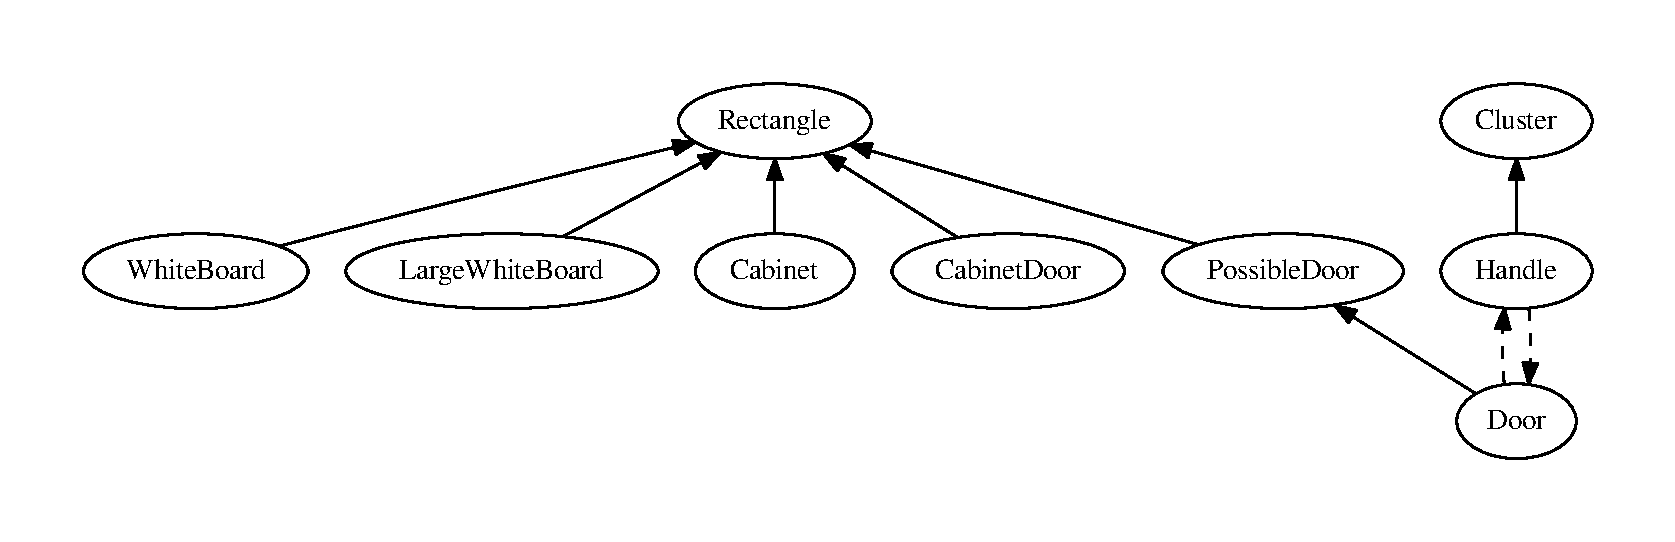
\includegraphics[width=\textwidth]{diagrammi/classifier}
  \caption{Grafo delle dipendenze}
  \label{fig:grafo-dipendenze}
\end{figure}

\begin{figure}[ht]
  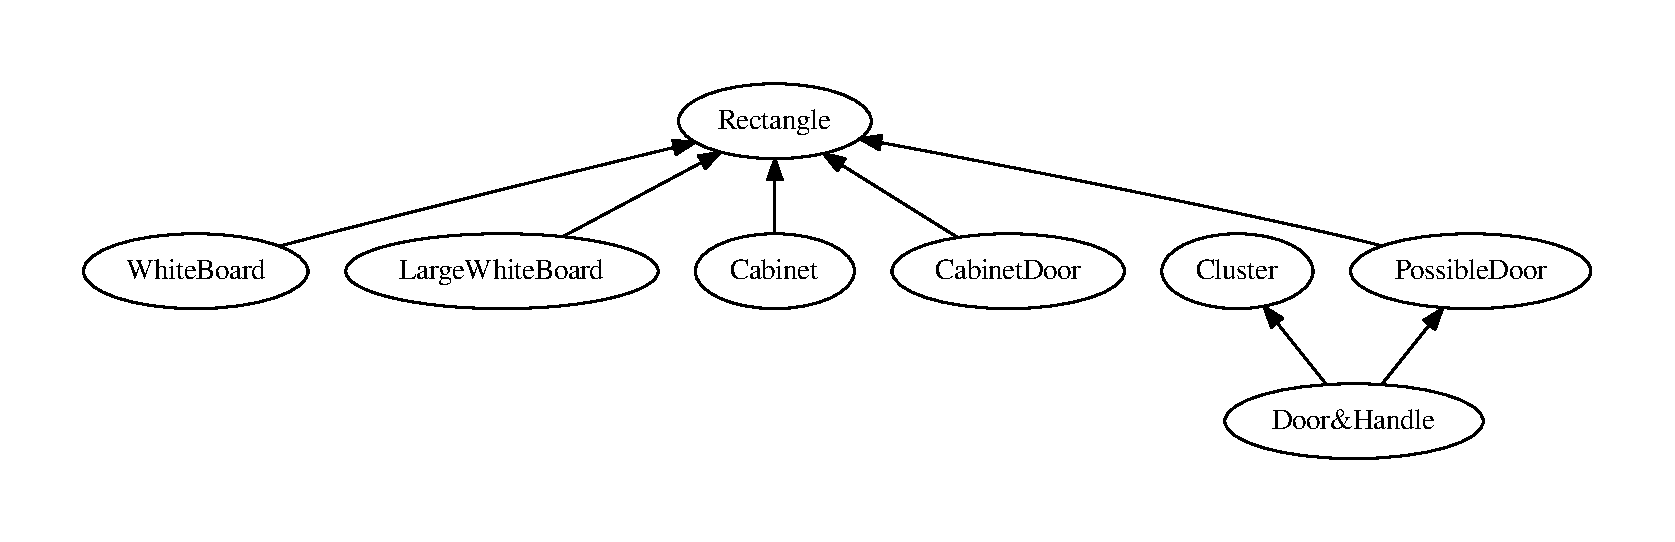
\includegraphics[width=\textwidth]{diagrammi/reasoning}
  \caption{Grafo di reasoning}
  \label{fig:grafo-reasoning}
\end{figure}


\end{document}
